\documentclass[11pt,fleqn]{book} % Default font size and left-justified equations


%%%%%%%%%%%%%%%%%%%%%%%%%%%%%%%%%%%%%%%%%
% The Legrand Orange Book
% Structural Definitions File
% Version 2.0 (9/2/15)
%
% Original author:
% Mathias Legrand (legrand.mathias@gmail.com) with modifications by:
% Vel (vel@latextemplates.com)
% 
% This file has been downloaded from:
% http://www.LaTeXTemplates.com
%
% License:
% CC BY-NC-SA 3.0 (http://creativecommons.org/licenses/by-nc-sa/3.0/)
%
%%%%%%%%%%%%%%%%%%%%%%%%%%%%%%%%%%%%%%%%%

%----------------------------------------------------------------------------------------
%	VARIOUS REQUIRED PACKAGES AND CONFIGURATIONS
%----------------------------------------------------------------------------------------

\usepackage[top=3cm,bottom=3cm,left=3cm,right=3cm,headsep=10pt,a4paper]{geometry} % Page margins

\usepackage{graphicx} % Required for including pictures
\graphicspath{{images/}} % Specifies the directory where pictures are stored

\usepackage{lipsum} % Inserts dummy text

\usepackage{tikz} % Required for drawing custom shapes

\usepackage[english]{babel} % English language/hyphenation

\usepackage{enumitem} % Customize lists
\setlist{nolistsep} % Reduce spacing between bullet points and numbered lists

\usepackage{booktabs} % Required for nicer horizontal rules in tables

\usepackage{xcolor} % Required for specifying colors by name
\definecolor{ocre}{RGB}{243,102,25} % Define the orange color used for highlighting throughout the book

%----------------------------------------------------------------------------------------
%	FONTS
%----------------------------------------------------------------------------------------

\usepackage{avant} % Use the Avantgarde font for headings
%\usepackage{times} % Use the Times font for headings
\usepackage{mathptmx} % Use the Adobe Times Roman as the default text font together with math symbols from the Sym­bol, Chancery and Com­puter Modern fonts

\usepackage{microtype} % Slightly tweak font spacing for aesthetics
\usepackage[utf8]{inputenc} % Required for including letters with accents
\usepackage[T1]{fontenc} % Use 8-bit encoding that has 256 glyphs

%----------------------------------------------------------------------------------------
%	BIBLIOGRAPHY AND INDEX
%----------------------------------------------------------------------------------------

\usepackage[style=alphabetic,citestyle=numeric,sorting=nyt,sortcites=true,autopunct=true,babel=hyphen,hyperref=true,abbreviate=false,backref=true,backend=biber]{biblatex}
\addbibresource{bibliography.bib} % BibTeX bibliography file
\defbibheading{bibempty}{}

\usepackage{calc} % For simpler calculation - used for spacing the index letter headings correctly
\usepackage{makeidx} % Required to make an index
\makeindex % Tells LaTeX to create the files required for indexing

%----------------------------------------------------------------------------------------
%	MAIN TABLE OF CONTENTS
%----------------------------------------------------------------------------------------

\usepackage{titletoc} % Required for manipulating the table of contents

\contentsmargin{0cm} % Removes the default margin

% Part text styling
\titlecontents{part}[0cm]
{\addvspace{20pt}\centering\large\bfseries}
{}
{}
{}

% Chapter text styling
\titlecontents{chapter}[1.25cm] % Indentation
{\addvspace{12pt}\large\sffamily\bfseries} % Spacing and font options for chapters
{\color{ocre!60}\contentslabel[\Large\thecontentslabel]{1.25cm}\color{ocre}} % Chapter number
{\color{ocre}}  
{\color{ocre!60}\normalsize\;\titlerule*[.5pc]{.}\;\thecontentspage} % Page number

% Section text styling
\titlecontents{section}[1.25cm] % Indentation
{\addvspace{3pt}\sffamily\bfseries} % Spacing and font options for sections
{\contentslabel[\thecontentslabel]{1.25cm}} % Section number
{}
{\hfill\color{black}\thecontentspage} % Page number
[]

% Subsection text styling
\titlecontents{subsection}[1.25cm] % Indentation
{\addvspace{1pt}\sffamily\small} % Spacing and font options for subsections
{\contentslabel[\thecontentslabel]{1.25cm}} % Subsection number
{}
{\ \titlerule*[.5pc]{.}\;\thecontentspage} % Page number
[]

% List of figures
\titlecontents{figure}[0em]
{\addvspace{-5pt}\sffamily}
{\thecontentslabel\hspace*{1em}}
{}
{\ \titlerule*[.5pc]{.}\;\thecontentspage}
[]

% List of tables
\titlecontents{table}[0em]
{\addvspace{-5pt}\sffamily}
{\thecontentslabel\hspace*{1em}}
{}
{\ \titlerule*[.5pc]{.}\;\thecontentspage}
[]

%----------------------------------------------------------------------------------------
%	MINI TABLE OF CONTENTS IN PART HEADS
%----------------------------------------------------------------------------------------

% Chapter text styling
\titlecontents{lchapter}[0em] % Indenting
{\addvspace{15pt}\large\sffamily\bfseries} % Spacing and font options for chapters
{\color{ocre}\contentslabel[\Large\thecontentslabel]{1.25cm}\color{ocre}} % Chapter number
{}  
{\color{ocre}\normalsize\sffamily\bfseries\;\titlerule*[.5pc]{.}\;\thecontentspage} % Page number

% Section text styling
\titlecontents{lsection}[0em] % Indenting
{\sffamily\small} % Spacing and font options for sections
{\contentslabel[\thecontentslabel]{1.25cm}} % Section number
{}
{}

% Subsection text styling
\titlecontents{lsubsection}[.5em] % Indentation
{\normalfont\footnotesize\sffamily} % Font settings
{}
{}
{}

%----------------------------------------------------------------------------------------
%	PAGE HEADERS
%----------------------------------------------------------------------------------------

\usepackage{fancyhdr} % Required for header and footer configuration

\pagestyle{fancy}
\renewcommand{\chaptermark}[1]{\markboth{\sffamily\normalsize\bfseries\chaptername\ \thechapter.\ #1}{}} % Chapter text font settings
\renewcommand{\sectionmark}[1]{\markright{\sffamily\normalsize\thesection\hspace{5pt}#1}{}} % Section text font settings
\fancyhf{} \fancyhead[LE,RO]{\sffamily\normalsize\thepage} % Font setting for the page number in the header
\fancyhead[LO]{\rightmark} % Print the nearest section name on the left side of odd pages
\fancyhead[RE]{\leftmark} % Print the current chapter name on the right side of even pages
\renewcommand{\headrulewidth}{0.5pt} % Width of the rule under the header
\addtolength{\headheight}{2.5pt} % Increase the spacing around the header slightly
\renewcommand{\footrulewidth}{0pt} % Removes the rule in the footer
\fancypagestyle{plain}{\fancyhead{}\renewcommand{\headrulewidth}{0pt}} % Style for when a plain pagestyle is specified

% Removes the header from odd empty pages at the end of chapters
\makeatletter
\renewcommand{\cleardoublepage}{
\clearpage\ifodd\c@page\else
\hbox{}
\vspace*{\fill}
\thispagestyle{empty}
\newpage
\fi}

%----------------------------------------------------------------------------------------
%	THEOREM STYLES
%----------------------------------------------------------------------------------------


\usepackage{amsmath,amsfonts,amssymb,amsthm,mathtools} % For math equations, theorems, symbols, etc
\DeclarePairedDelimiter\ceil{\lceil}{\rceil}
\DeclarePairedDelimiter\floor{\lfloor}{\rfloor}

\newcommand{\intoo}[2]{\mathopen{]}#1\,;#2\mathclose{[}}
\newcommand{\ud}{\mathop{\mathrm{{}d}}\mathopen{}}
\newcommand{\intff}[2]{\mathopen{[}#1\,;#2\mathclose{]}}
\newtheorem{notation}{Notation}[chapter]

% Boxed/framed environments
\newtheoremstyle{ocrenumbox}% % Theorem style name
{0pt}% Space above
{0pt}% Space below
{\normalfont}% % Body font
{}% Indent amount
{\small\bf\sffamily\color{ocre}}% % Theorem head font
{\;}% Punctuation after theorem head
{0.25em}% Space after theorem head
{\small\sffamily\color{ocre}\thmname{#1}\nobreakspace\thmnumber{\@ifnotempty{#1}{}\@upn{#2}}% Theorem text (e.g. Theorem 2.1)
\thmnote{\nobreakspace\the\thm@notefont\sffamily\bfseries\color{black}---\nobreakspace#3.}} % Optional theorem note
\renewcommand{\qedsymbol}{$\blacksquare$}% Optional qed square

\newtheoremstyle{blacknumex}% Theorem style name
{5pt}% Space above
{5pt}% Space below
{\normalfont}% Body font
{} % Indent amount
{\small\bf\sffamily}% Theorem head font
{\;}% Punctuation after theorem head
{0.25em}% Space after theorem head
{\small\sffamily{\tiny\ensuremath{\blacksquare}}\nobreakspace\thmname{#1}\nobreakspace\thmnumber{\@ifnotempty{#1}{}\@upn{#2}}% Theorem text (e.g. Theorem 2.1)
\thmnote{\nobreakspace\the\thm@notefont\sffamily\bfseries---\nobreakspace#3.}}% Optional theorem note

\newtheoremstyle{blacknumbox} % Theorem style name
{0pt}% Space above
{0pt}% Space below
{\normalfont}% Body font
{}% Indent amount
{\small\bf\sffamily}% Theorem head font
{\;}% Punctuation after theorem head
{0.25em}% Space after theorem head
{\small\sffamily\thmname{#1}\nobreakspace\thmnumber{\@ifnotempty{#1}{}\@upn{#2}}% Theorem text (e.g. Theorem 2.1)
\thmnote{\nobreakspace\the\thm@notefont\sffamily\bfseries---\nobreakspace#3.}}% Optional theorem note

% Non-boxed/non-framed environments
\newtheoremstyle{ocrenum}% % Theorem style name
{5pt}% Space above
{5pt}% Space below
{\normalfont}% % Body font
{}% Indent amount
{\small\bf\sffamily\color{ocre}}% % Theorem head font
{\;}% Punctuation after theorem head
{0.25em}% Space after theorem head
{\small\sffamily\color{ocre}\thmname{#1}\nobreakspace\thmnumber{\@ifnotempty{#1}{}\@upn{#2}}% Theorem text (e.g. Theorem 2.1)
\thmnote{\nobreakspace\the\thm@notefont\sffamily\bfseries\color{black}---\nobreakspace#3.}} % Optional theorem note
\renewcommand{\qedsymbol}{$\blacksquare$}% Optional qed square
\makeatother

% Defines the theorem text style for each type of theorem to one of the three styles above
\newcounter{dummy} 
\numberwithin{dummy}{section}
\theoremstyle{ocrenumbox}
\newtheorem{theoremeT}[dummy]{Theorem}

\newtheorem{problem}{Exercise}[chapter]
\theoremstyle{blacknumex}
\newtheorem{solution}{Solution}[chapter]
\theoremstyle{blacknumex}
\newtheorem{exampleT}{Example}[chapter]
\theoremstyle{blacknumbox}
\newtheorem{vocabulary}{Vocabulary}[chapter]
\newtheorem{definitionT}{Definition}[section]
\newtheorem{corollaryT}[dummy]{Corollary}
\theoremstyle{ocrenum}
\newtheorem{proposition}[dummy]{Proposition}

%----------------------------------------------------------------------------------------
%	DEFINITION OF COLORED BOXES
%----------------------------------------------------------------------------------------

\RequirePackage[framemethod=default]{mdframed} % Required for creating the theorem, definition, exercise and corollary boxes

% Theorem box
\newmdenv[skipabove=7pt,
skipbelow=7pt,
backgroundcolor=black!5,
linecolor=ocre,
innerleftmargin=5pt,
innerrightmargin=5pt,
innertopmargin=5pt,
leftmargin=0cm,
rightmargin=0cm,
innerbottommargin=5pt]{tBox}

% Exercise box	  
\newmdenv[skipabove=7pt,
skipbelow=7pt,
rightline=false,
leftline=true,
topline=false,
bottomline=false,
backgroundcolor=ocre!10,
linecolor=ocre,
innerleftmargin=5pt,
innerrightmargin=5pt,
innertopmargin=5pt,
innerbottommargin=5pt,
leftmargin=0cm,
rightmargin=0cm,
linewidth=4pt]{eBox}	

% Definition box
\newmdenv[skipabove=7pt,
skipbelow=7pt,
rightline=false,
leftline=true,
topline=false,
bottomline=false,
linecolor=ocre,
innerleftmargin=5pt,
innerrightmargin=5pt,
innertopmargin=0pt,
leftmargin=0cm,
rightmargin=0cm,
linewidth=4pt,
innerbottommargin=0pt]{dBox}	

% Corollary box
\newmdenv[skipabove=7pt,
skipbelow=7pt,
rightline=false,
leftline=true,
topline=false,
bottomline=false,
linecolor=gray,
backgroundcolor=black!5,
innerleftmargin=5pt,
innerrightmargin=5pt,
innertopmargin=5pt,
leftmargin=0cm,
rightmargin=0cm,
linewidth=4pt,
innerbottommargin=5pt]{cBox}

% Creates an environment for each type of theorem and assigns it a theorem text style from the "Theorem Styles" section above and a colored box from above
\newenvironment{theorem}{\begin{tBox}\begin{theoremeT}}{\end{theoremeT}\end{tBox}}
\newenvironment{exercise}{\begin{eBox}\begin{exerciseT}}{\hfill{\color{ocre}\tiny\ensuremath{\blacksquare}}\end{exerciseT}\end{eBox}}				  
\newenvironment{definition}{\begin{dBox}\begin{definitionT}}{\end{definitionT}\end{dBox}}	
\newenvironment{example}{\begin{exampleT}}{\hfill{\tiny\ensuremath{\blacksquare}}\end{exampleT}}		
\newenvironment{corollary}{\begin{cBox}\begin{corollaryT}}{\end{corollaryT}\end{cBox}}	

%----------------------------------------------------------------------------------------
%	REMARK ENVIRONMENT
%----------------------------------------------------------------------------------------

\newenvironment{remark}{\par\vspace{10pt}\small % Vertical white space above the remark and smaller font size
\begin{list}{}{
\leftmargin=35pt % Indentation on the left
\rightmargin=25pt}\item\ignorespaces % Indentation on the right
\makebox[-2.5pt]{\begin{tikzpicture}[overlay]
\node[draw=ocre!60,line width=1pt,circle,fill=ocre!25,font=\sffamily\bfseries,inner sep=2pt,outer sep=0pt] at (-15pt,0pt){\textcolor{ocre}{R}};\end{tikzpicture}} % Orange R in a circle
\advance\baselineskip -1pt}{\end{list}\vskip5pt} % Tighter line spacing and white space after remark

%----------------------------------------------------------------------------------------
%	SECTION NUMBERING IN THE MARGIN
%----------------------------------------------------------------------------------------

\makeatletter
\renewcommand{\@seccntformat}[1]{\llap{\textcolor{ocre}{\csname the#1\endcsname}\hspace{1em}}}                    
\renewcommand{\section}{\@startsection{section}{1}{\z@}
{-4ex \@plus -1ex \@minus -.4ex}
{1ex \@plus.2ex }
{\normalfont\large\sffamily\bfseries}}
\renewcommand{\subsection}{\@startsection {subsection}{2}{\z@}
{-3ex \@plus -0.1ex \@minus -.4ex}
{0.5ex \@plus.2ex }
{\normalfont\sffamily\bfseries}}
\renewcommand{\subsubsection}{\@startsection {subsubsection}{3}{\z@}
{-2ex \@plus -0.1ex \@minus -.2ex}
{.2ex \@plus.2ex }
{\normalfont\small\sffamily\bfseries}}                        
\renewcommand\paragraph{\@startsection{paragraph}{4}{\z@}
{-2ex \@plus-.2ex \@minus .2ex}
{.1ex}
{\normalfont\small\sffamily\bfseries}}

%----------------------------------------------------------------------------------------
%	PART HEADINGS
%----------------------------------------------------------------------------------------

% numbered part in the table of contents
\newcommand{\@mypartnumtocformat}[2]{%
\setlength\fboxsep{0pt}%
\noindent\colorbox{ocre!20}{\strut\parbox[c][.7cm]{\ecart}{\color{ocre!70}\Large\sffamily\bfseries\centering#1}}\hskip\esp\colorbox{ocre!40}{\strut\parbox[c][.7cm]{\linewidth-\ecart-\esp}{\Large\sffamily\centering#2}}}%
%%%%%%%%%%%%%%%%%%%%%%%%%%%%%%%%%%
% unnumbered part in the table of contents
\newcommand{\@myparttocformat}[1]{%
\setlength\fboxsep{0pt}%
\noindent\colorbox{ocre!40}{\strut\parbox[c][.7cm]{\linewidth}{\Large\sffamily\centering#1}}}%
%%%%%%%%%%%%%%%%%%%%%%%%%%%%%%%%%%
\newlength\esp
\setlength\esp{4pt}
\newlength\ecart
\setlength\ecart{1.2cm-\esp}
\newcommand{\thepartimage}{}%
\newcommand{\partimage}[1]{\renewcommand{\thepartimage}{#1}}%
\def\@part[#1]#2{%
\ifnum \c@secnumdepth >-2\relax%
\refstepcounter{part}%
\addcontentsline{toc}{part}{\texorpdfstring{\protect\@mypartnumtocformat{\thepart}{#1}}{\partname~\thepart\ ---\ #1}}
\else%
\addcontentsline{toc}{part}{\texorpdfstring{\protect\@myparttocformat{#1}}{#1}}%
\fi%
\startcontents%
\markboth{}{}%
{\thispagestyle{empty}%
\begin{tikzpicture}[remember picture,overlay]%
\node at (current page.north west){\begin{tikzpicture}[remember picture,overlay]%	
\fill[ocre!20](0cm,0cm) rectangle (\paperwidth,-\paperheight);
\node[anchor=north] at (4cm,-3.25cm){\color{ocre!40}\fontsize{220}{100}\sffamily\bfseries\@Roman\c@part}; 
\node[anchor=south east] at (\paperwidth-1cm,-\paperheight+1cm){\parbox[t][][t]{8.5cm}{
\printcontents{l}{0}{\setcounter{tocdepth}{1}}%
}};
\node[anchor=north east] at (\paperwidth-1.5cm,-3.25cm){\parbox[t][][t]{15cm}{\strut\raggedleft\color{white}\fontsize{30}{30}\sffamily\bfseries#2}};
\end{tikzpicture}};
\end{tikzpicture}}%
\@endpart}
\def\@spart#1{%
\startcontents%
\phantomsection
{\thispagestyle{empty}%
\begin{tikzpicture}[remember picture,overlay]%
\node at (current page.north west){\begin{tikzpicture}[remember picture,overlay]%	
\fill[ocre!20](0cm,0cm) rectangle (\paperwidth,-\paperheight);
\node[anchor=north east] at (\paperwidth-1.5cm,-3.25cm){\parbox[t][][t]{15cm}{\strut\raggedleft\color{white}\fontsize{30}{30}\sffamily\bfseries#1}};
\end{tikzpicture}};
\end{tikzpicture}}
\addcontentsline{toc}{part}{\texorpdfstring{%
\setlength\fboxsep{0pt}%
\noindent\protect\colorbox{ocre!40}{\strut\protect\parbox[c][.7cm]{\linewidth}{\Large\sffamily\protect\centering #1\quad\mbox{}}}}{#1}}%
\@endpart}
\def\@endpart{\vfil\newpage
\if@twoside
\if@openright
\null
\thispagestyle{empty}%
\newpage
\fi
\fi
\if@tempswa
\twocolumn
\fi}

%----------------------------------------------------------------------------------------
%	CHAPTER HEADINGS
%----------------------------------------------------------------------------------------

% A switch to conditionally include a picture, implemented by  Christian Hupfer
\newif\ifusechapterimage
\usechapterimagetrue
\newcommand{\thechapterimage}{}%
\newcommand{\chapterimage}[1]{\ifusechapterimage\renewcommand{\thechapterimage}{#1}\fi}%
\def\@makechapterhead#1{%
{\parindent \z@ \raggedright \normalfont
\ifnum \c@secnumdepth >\m@ne
\if@mainmatter
\begin{tikzpicture}[remember picture,overlay]
\node at (current page.north west)
{\begin{tikzpicture}[remember picture,overlay]
\node[anchor=north west,inner sep=0pt] at (0,0) {\ifusechapterimage\includegraphics[width=\paperwidth]{\thechapterimage}\fi};
\draw[anchor=west] (\Gm@lmargin,-9cm) node [line width=2pt,rounded corners=15pt,draw=ocre,fill=white,fill opacity=0.5,inner sep=15pt]{\strut\makebox[22cm]{}};
\draw[anchor=west] (\Gm@lmargin+.3cm,-9cm) node {\huge\sffamily\bfseries\color{black}\thechapter. #1\strut};
\end{tikzpicture}};
\end{tikzpicture}
\else
\begin{tikzpicture}[remember picture,overlay]
\node at (current page.north west)
{\begin{tikzpicture}[remember picture,overlay]
\node[anchor=north west,inner sep=0pt] at (0,0) {\ifusechapterimage\includegraphics[width=\paperwidth]{\thechapterimage}\fi};
\draw[anchor=west] (\Gm@lmargin,-9cm) node [line width=2pt,rounded corners=15pt,draw=ocre,fill=white,fill opacity=0.5,inner sep=15pt]{\strut\makebox[22cm]{}};
\draw[anchor=west] (\Gm@lmargin+.3cm,-9cm) node {\huge\sffamily\bfseries\color{black}#1\strut};
\end{tikzpicture}};
\end{tikzpicture}
\fi\fi\par\vspace*{270\p@}}}

%-------------------------------------------

\def\@makeschapterhead#1{%
\begin{tikzpicture}[remember picture,overlay]
\node at (current page.north west)
{\begin{tikzpicture}[remember picture,overlay]
\node[anchor=north west,inner sep=0pt] at (0,0) {\ifusechapterimage\includegraphics[width=\paperwidth]{\thechapterimage}\fi};
\draw[anchor=west] (\Gm@lmargin,-9cm) node [line width=2pt,rounded corners=15pt,draw=ocre,fill=white,fill opacity=0.5,inner sep=15pt]{\strut\makebox[22cm]{}};
\draw[anchor=west] (\Gm@lmargin+.3cm,-9cm) node {\huge\sffamily\bfseries\color{black}#1\strut};
\end{tikzpicture}};
\end{tikzpicture}
\par\vspace*{270\p@}}
\makeatother

%----------------------------------------------------------------------------------------
%	HYPERLINKS IN THE DOCUMENTS
%----------------------------------------------------------------------------------------

\usepackage{hyperref}
\hypersetup{hidelinks,backref=true,pagebackref=true,hyperindex=true,colorlinks=false,breaklinks=true,urlcolor= ocre,bookmarks=true,bookmarksopen=false,pdftitle={Title},pdfauthor={Author}}
\usepackage{bookmark}
\bookmarksetup{
open,
numbered,
addtohook={%
\ifnum\bookmarkget{level}=0 % chapter
\bookmarksetup{bold}%
\fi
\ifnum\bookmarkget{level}=-1 % part
\bookmarksetup{color=ocre,bold}%
\fi
}
}

%----------------------------------------------------------------------------------------
%	LISTINGS
%----------------------------------------------------------------------------------------
\usepackage{listings}
\lstset{language=C}
\lstset{
  basicstyle=\footnotesize\ttfamily,
  breaklines=true,
  showstringspaces=false,
  numbers=left,
  backgroundcolor=\color{bgcolor},
  commentstyle=\color{gray},
  keywordstyle=\color{blue},
  keywordstyle=[2]\color{teal},   % cyan or teal can also be a good choice, use \bfseries for bold
  frame=none,                     % adds a frame around the code
  tabsize=2,                      % sets default tabsize to 2 spaces
  captionpos=b,                   % sets the caption-position to bottom
  morekeywords=[2]{}              % if you want to add more keywords to the set
    __
}

\usepackage{color}
\definecolor{bgcolor}{rgb}{0.98,0.98,0.98}


%----------------------------------------------------------------------------------------
%	ALGORITHM
%----------------------------------------------------------------------------------------
\usepackage[]{algorithm2e}


\usepackage{mdframed,framed}



\begin{document}

%\frontmatter

\thispagestyle{empty}

\newcommand{\HS}[1][1.]{\hspace{\stretch{#1}}}
\begin{center}

%\begin{figure}
%\centerline{\psfig{figure=logouni.eps}}
%\end{figure}

\huge{UNIVERSITY OF CALABRIA}\\
\vspace*{0.25cm}
\large{Department of Mathematics and Computer Science}\\
\normalsize{Via P. Bucci\\
I-87036 Rende, Italy\\
\vspace*{0.25cm} \HS \hrulefill \HS}

%\large{Internal Report 02/2009}\\


\vspace*{3.5cm}

\Huge{\textbf{Google Interview Preparation Guide}}\\
\vspace*{0.2cm}
\large{\textbf{}}\\
\vspace*{0.7cm}
\Large{\textit{www.davidespataro.it}}
\vspace*{1cm}

%\normalsize{by}

\vspace*{1cm}

\normalsize{\textit{Davide Spataro}}

\vspace*{3.5cm}

\normalsize{May, 2016}

\vspace*{2.0cm}

%\footnotesize{This work was supported by the Department of Mathematics of
% University of Calabria. Parallel computer machineries were provided by the High Performance Computing Center of the same University.}

%\HS[.1] \hrulefill \hspace*{1.5cm} \\
%\quad \normalsize A.A. 2002-2003 \quad

\end{center}


%----------------------------------------------------------------------------------------
%	TABLE OF CONTENTS
%----------------------------------------------------------------------------------------

%\usechapterimagefalse % If you don't want to include a chapter image, use this to toggle images off - it can be enabled later with \usechapterimagetrue

\chapterimage{ch4} % Table of contents heading image

\pagestyle{empty} % No headers

\tableofcontents % Print the table of contents itself

\cleardoublepage % Forces the first chapter to start on an odd page so it's on the right

\pagestyle{fancy} % Print headers again


%
\chapter{Primitive Data Types}

\section{Boolean}
\iffalse
https://oopscenities.net/2011/09/28/c-primitive-types/
https://en.wikipedia.org/wiki/Primitive_data_type
http://rypress.com/tutorials/objective-c/data-types/primitives
https://en.wikipedia.org/wiki/C_data_types
\fi
\section{Character}

\section{Floating-point}

\section{Integer}

\section{Enumeration}


\chapter{Composite Data Types}
\section{Record - struct or class}
\section{Union}
\section{Tagged Union}


\chapter{Array}
Array belongs to the so called \textit{Contiguous} Data Structure in which stored elements (all of the same type) are arranged in a \textbf{single} slab of memory. Array's elements can be easily  accessed given their \textit{indices} within the array itself the same way, using an analogy, we can locate an house in a specific street given its postcode. Array can also be tought as a collection of variables of the same type.

Major characteristic of arrays are:
\begin{description}
\item [Constant time access] All the element of the array can be accessed in $\mathcal{O}(1)$. Array can be fully described by its
	\begin{enumerate}
		\item Starting address $m_0$
		\item Size of Stored data type (e.g. 4 bytes for \texttt{int} or 1 byte for \texttt{char}) $S$
		\item Number of stored elements (i.e. array length) $L$
	\end{enumerate}
	\begin{figure}[h]
		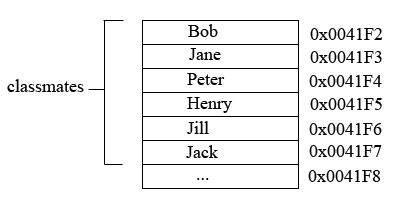
\includegraphics[width=8cm]{array1.png}
	\end{figure}
	The starting address correnspond to the first element (in C-like languages index $0$) element.
	 The second element starts at the address  $m_0 + S$, third at $m_0 + S + S$ and so on. so the element at index $i$ has index $s_i = m_0 +iS$.
	
\item [Only Data] Array are space efficient because they do not store any other information but data itself (unlike list for instance where each node of the list stores a pointer to the next element of the list). 
 
\item [Memory locality] Array adhere perfectly to the principle of spatial locality\footnote{If a particular memory location is referenced at a particular time, then it is likely that nearby memory locations will be referenced in the near future. In this case it is common to attempt to guess the size and shape of the area around the current reference for which it is worthwhile to prepare faster access.} in which related storage locations are frequently accessed (iterating through an array is a very common idiom in all programming languages). This allows cache to work at his best.
\end{description}

Arrays have fixed size, and this in several application is a major downside (the size of the array is input dependent for instance). C-like languages allow for dynamic memory allocation at runtime (see \ref{chap:malloc} at page (\pageref{{chap;malloc}}). This involves the creation of a (different) larger (how larger is an important point) array and the copy of the first one in the beginning of the newly created one. If the program requires this dynamic enlarging often we could end up wasting much time in copying data here and there.
The common strategy used for creating a dynamic array is to double the size of the array each time. This mitigate the average number of copies of each element. Let's imagine we start with an array of size one and we try to insert $n$ elements, doubling the size of the array when its capacity its full. The first element is has to be copied when the array expands after the fist, second, fourth, eighth ... $2^i = n$ insertion.
It will take $i = log(n)$ doubling size for the array to have size $n$. Element in the last half of the array will be copied only one (at the last doubling). A quarter of the elements will be copied twic and so on. The total number of copies will be then
\[
M = \sum_{i=1}^{\log(n)} \frac{ni}{2^i} = n\sum_{i=1}^{\log(n)} \frac{i}{2^i} = n(\frac{1}{2}+\frac{1}{2} + \frac{3}{8} + \frac{1}{3} ... \frac{log(n)}{n})=2n
\]
So in average  each element is copied only two times.

 \section{Problems and Solution}

%---Problem---------------------------------
\begin{problem}
Given an array, $A$, of $N$ integers, print each element in reverse order as a single line of space-separated integers.
\end{problem}	

\begin{solution}

		\begin{lstlisting}[language=C, caption="C"]
        int main(){
    int n; 
    scanf("%d",&n);
    int *arr = malloc(sizeof(int) * n);
    for(int arr_i = 0; arr_i < n; arr_i++){
       scanf("%d",&arr[arr_i]);
    }
    while(--n >=0){
       printf("%i ",arr[n]);
    }
    
    return 0;
}

		\end{lstlisting}  

\end{solution}	
%------------------------------------------------ 
 
  \begin{problem}
	Reverse an array in place.
 \end{problem}
 
 \begin{problem}
    Implement a function to determine if a string has all unique characters. String can only contains latin 	characters. What happen if you are forced to use no additional data structures?
\end{problem}

 \begin{problem}
    Implement a function to determine if a string has all unique characters. String can only contains latin 	characters. What happen if you are forced to use no additional data structures?
\end{problem}

 \begin{problem}
    Implement a function to determine the number of repeated characters in a string. (e.g. google has 2 repeated characters, \textit{g} and \textit{o}).
\end{problem}

 \begin{problem}
   Given an array of integer of given size containing numbers from 1 to $N \geq 2$ . Only one number is missing within the array. Write a function which output is that missing number.
\end{problem}

 \begin{problem}
   Given an array of integer of size $N$ containing numbers from 1 to $N-2$. All numbers appear only once except one which is repeated twice. Write a function which return that number.
\end{problem}

 \begin{problem}
Write a function which find the smallest and largest number in an unsorted array of integers. 
\end{problem}

 \begin{problem}
	Sort an array of integer using a $\mathcal{O}(n^2)$  and a $\mathcal{O}(nlog(n))$  algorithm. Both algorithm should sort the array \textit{in-place}.
\end{problem}

 \begin{problem}
	Given two array of sorted integer, \textit{A,B} find their intersection i.e. an array $C$ which contains only elements which belong both to A and B. $C=\{c_i \;|\; c_i \in A;,\; c_i \in B\}$
\end{problem}

 \begin{problem}
	Given two array of unsorted integer in which only one element is repeted (the rest of them appear only once). Write a function which finds that element in $\mathcal{O}(n)$  time.
\end{problem}

 \begin{problem}
	Write a function which finds the kth largest element in a unsorted array.
\end{problem}
 \begin{problem}
	Write a function which finds the kth smallest element in a unsorted array.
\end{problem}

 \begin{problem}
Count the number of distinct ( (a,b) is not distinct from (b,a) ) pairs in an array of integers which sum is equal to a given value $K$.
\end{problem}

 \begin{problem}
Given three sorted array (in non decreasing order) find the intersection between all of their elements.
\end{problem}

 \begin{problem}
Given an array, find the first repeated element. i.e. an element $e$ which occurs more than once and which index is the smallest. On the following input $1,2,3,4,5,3,2,2,7$ the function should return two because is the a repeated element with the smallest index (1).
\end{problem}

 \begin{problem}
Given an array, return the larger and the 2th-largst element.
\end{problem}


 \begin{problem}
Given an array of integer, find the smallest positive integer which cannot be represented as sum of any subset of the array. On  input 1, 3, 6, 10, 11, 15 the function should return 2. Note that the array can also contains negative numbers.
\end{problem}

 \begin{problem}
Given an array of integer (positive and negative), return an array which elements are rearranged in alternating positive and negative. You are ensured that the number of positives and negatives matches. E.g. on input $(1,2,-6,4,8,-6,-5)$ the functions (only one of the possible valide output) return $(1,-6,2,-6,4,-5,8)$.
\end{problem}

 \begin{problem}
Given an array of integer write a function which return true is a non empty subset of its element which sum up to $0$. False otherwise. 
\end{problem}

 \begin{problem}
Given an array $A$ of integer find the length of the  longest sequence of consecutive integers. On input $1,56,8,-5,3,7,4,23,2,5)$ the function should return 5 (is the length of the consecutive subsequence $(1,2,3,4,5)$)
 \end{problem}

 \begin{problem}
Find the minimum in a rotated sorted array. (a rotation of $1,2,3,4,5,6$ could be for instance $4,5,6,1,2,3$). The array does not contains duplicates.

What if we allows for duplicated to be present? How does this changes the overall time complexity?
 \end{problem}

 \begin{problem}\label{array:anagram}
Given two string, determine which is the minimum number of deletions (a delete operation can be performed on both string) necessary for the two string to be a valid anagram\footnote{A word, phrase, or name formed by rearranging the letters of another, such as spar, formed from rasp.} of each other. Strings contains only latin characters with no space. Given \textit{hello} and \textit{belloz} the function should returns 2. ( See solution \ref{array:anagram_sol} at page \pageref{array:anagram_sol} )


\begin{lstlisting}[ label=array:anagram_sol, caption=Solution to problem \ref{array:anagram} ]
#include <stdio.h>
#include <string.h>
#include <math.h>
#include <stdlib.h>

void removeTrailingNL(char* s){
    int size = strlen(s);
    if(size > 0 && s[size-1] == '\n')
        s[size-1] = '\0';
}

#define MAX_INPUT_SIZE (10000)
int main() {
    const int alph_size = 'z'-'a'+1;
    int s1_freq[alph_size];
    int s2_freq[alph_size];
    //initialize frequencies arrays
    for(int i = 0 ; i < alph_size ; i++){
        s1_freq[i] = 0;
        s2_freq[i] = 0;
    }
    //read both string
    char s1[10000];
    char s2[10000];
    fgets(s1,MAX_INPUT_SIZE,stdin);
    fgets(s2,MAX_INPUT_SIZE,stdin);
    removeTrailingNL(s1);
    removeTrailingNL(s2);
    
    int size_s1, size_s2;
    size_s1 = strlen(s1);
    size_s2 = strlen(s2);
    //compute frequencies
    for(int i  = 0 ; i< size_s1 ; i++)
        s1_freq[s1[i]-'a'] = s1_freq[s1[i]-'a'] + 1;
    for(int i  = 0 ; i< size_s2 ; i++)
        s2_freq[s2[i]-'a'] = s2_freq[s2[i]-'a'] + 1;
    /*
  //print frequencies  
 for(int i  = 0 ; i< alph_size ; i++){
     printf("%c %i %i\n",'a'+i,s1_freq[i],s2_freq[i]);
 }*/
    
    //compute minimum delete operation
    int dels = 0;
    for(int i  = 0 ; i< alph_size ; i++)
        dels = dels + (abs(s1_freq[i] - s2_freq[i]));
    
    
    //prints output
    printf("%i",dels);
   
    return 0;
}
\end{lstlisting}
 \end{problem}






\chapter{List}
\section{Singly Linked List}
\section{Doubly Linked List}
\section{Circular Linked List}
\section{Self-Organizing Lists}
\section{Skip Lists}

\chapter{Stack}

\chapter{Queue}
\section{Double-ended queue - Dequeue}

\section{Priority Queue}
Nevertheless, the heap data structure itself has enormous utility. In this section, we present one of the most popular applications of a heap: its use as an efficient priority queue.
A priority queue is a data structure for maintaining a set S of elements, each with an associated value called a key. A priority queue supports the following operations.
\begin{description}
\item [\texttt{INSERT(S,x)}] inserts an element $x$ into the set S
\item [\texttt{\{MAX,MIN\}(S,x)}] return the element of S with largest/smallest key 
\item [\texttt{EXTRACT-\{MAX,MIN\}(S,x)}] return and removes the element of S with largest/smallest key 
\end{description}
One application of priority queues is to schedule jobs on a shared computer. The priority queue keeps track of the jobs to be performed and their relative priorities. When a job is finished or interrupted, the highest-priority job is selected from those pending using EXTRACT-MAX. A new job can be added to the queue at any time using INSERT.

A priority queue can also be used in an event-driven simulator. The items in the queue are events to be simulated, each with an associated time of occurrence that serves as its key. The events must be simulated in order of their time of occurrence, because the simulation of an event can cause other events to be simulated in the future. For this application, it is natural to reverse the linear order of the priority queue and support the operations MINIMUM and EXTRACT-MIN instead of MAXIMUM and EXTRACT-MAX. The simulation program uses EXTRACT-MIN at each step to choose the next event to simulate. As new events are produced, they are inserted into the priority queue using INSERT.

Not surprisingly, we can use a heap to implement a priority queue. The operation HEAP-MAXIMUM returns the maximum heap element in (1) time by simply returning the value A[1] in the heap. The HEAP-EXTRACT-MAX procedure is similar to the for loop body (lines 3-5) of the HEAPSORT procedure:

\begin{algorithm}[H]
 \KwData{Heap H}
 \KwResult{Extract Max - Max element of H}
\uIf{heap-size(H) $<$ 1}{
	 underflow error
   }

$max \gets H[1]$\;
$H[1] \gets H[heap-size(H)]$\;
$heap-size(H) \gets heap-size(H) -1$\;
\Return{max}\;

\caption{Priority Queue Extract-max pseudocode}
\end{algorithm}

The running time of HEAP-EXTRACT-MAX is $\mathcal{O}(log n)$, since it performs only a constant amount of work on top of the $\mathcal{O}(log n)$ time for HEAPIFY.

The HEAP-INSERT procedure inserts a node into heap A. To do so, it first expands the heap by adding a new leaf to the tree. Then, in a manner reminiscent of the insertion loop of INSERTION-SORT (see section \ref{sec:insertionsort} at page \pageref{sec:insertionsort}), it traverses a path from this leaf toward the root to find a proper place for the new element.

\begin{algorithm}[H]
 \KwData{Heap H, Key key}
 \KwResult{Insert an element in the Heap H}
	$heap-size(H) \gets heap-size(H)+1$\;
	$i \gets heap-size(H)$\;
	\While{$i > 1 and H[parent(i)] < key$}{
		$H[i] \gets H[parent(i)]$\;
		$i \gets parent(i)$\;
	}
	$H[i] \gets key$
\caption{Priority Queue insert pseudocode}
\end{algorithm}

\begin{problem}
Show how to implement a first-in, first-out queue with a priority queue. Show how to implement a stack with a priority queue.
\end{problem}


\begin{problem}

Give an O(lg n)-time implementation of the procedure HEAP-INCREASE-KEY(A, i, k), which sets A[i]  max(A[i],k) and updates the heap structure appropriately.
\end{problem}

\begin{problem}

The operation HEAP-DELETE(A, i) deletes the item in node i from heap A. Give an implementation of HEAP-DELETE that runs in O(lg n) time for an n-element heap.
\end{problem}

\begin{problem}

Give an O(n lg k)-time algorithm to merge k sorted lists into one sorted list, where n is the total number of elements in all the input lists. (Hint: Use a heap for k-way merging.)
\end{problem}


\begin{problem}

A d-ary heap is like a binary heap, but instead of 2 children, nodes have d children.
\begin{enumerate}
\item How would you represent a d-ary heap in an array?
\item What is the height of a d-ary heap of n elements in terms of n and d?
\item Give an efficient implementation of EXTRACT-MAX. Analyze its running time in terms of d and n.
\item Give an efficient implementation of INSERT. Analyze its running time in terms of d and n.
\item Give an efficient implementation of HEAP-INCREASE-KEY(A, i, k), which sets A[i]  max(A[i], k) and updates the heap structure appropriately. Analyze its running time in terms of d and n.
\end{enumerate}
\end{problem}








\chapter{Heap}


\chapter{Tree}

\section{Binary Tree}
\section{Binary Search Tree}

\section{Self Balancing Tree}
\subsection{B Tree}
\subsection{B+ Tree}

\subsection{Adelson-Velsky Landis Tree - AVL Tree}
\subsection{Red Black Tree}
\subsection{Splay Tree}


\section{Space-partitioning trees}
\subsection{Kd Tree}
\subsection{R Tree}

%-----CHAPTER GRAPH---------------------------
\chapter{Graph}

\section{Visiting Algorithm}


\subsection{Depth-first}

\subsection{Breadth-first}

Given a graph $G = (V,E)$ and a distinguished source vertex $s$, breadth-first
search systematically explores the edges of $G$ to “discover” every vertex that is
reachable from $s$. It has the convenient property that in unweighted graph it computes the minimum distance from $s$ to all the node reachable from $s$ itself producing the so called breadth-first tree with root $s$. It takes its name from the fact that is first expand the frontier of the currently visited node. It first examine all the node at ditance $k$ from the root before to visit those at distance $k+1$.
Each node is labeled as undiscovered, discovered or processed, reflecting the different states in which a node can be during the visit.

The breadth tree is initially initialized with the root $s$. Then whenever the search encounter a undiscovered node $v$ it is inserted among those to be visited and labeled as discovered and the edge that lead from the examined node to $v$ is added to the breadth tree. Since we visit every node only once and for each node we examine its adjacency list in its full length the complexity is is $O(V+E)$


\subsection{Why Breadth-First computes the shortest path}
Let $\delta(s,u)$ be the shortest path (or minimum distance) between two vertices $s,v$\footnote{Note that for undirected graphs this distance is symmetric i.e. $\delta(s,u) = \delta(u,s)$}. If a path does not exists then $\delta(s,u) = \infty$. Note also that $\delta(s,s) = 0$. 
\begin{theorem}{Tringular inequality}
\label{theo:triangular_inequality}
The triangular inqeuality can be expressed using the following formula:
\[
\forall x,y,w \; |\; \delta(x,w) \leq   \delta(x,y) + \delta(y,w)
\]
It says that the shortest path between $x,w$ cannot is always equal or shorter than the path from from $x$ leads to $w$ passing from an intermediate node $y$ (see image \ref{fig:triangularinequality})\footnote{Is called triangular because is can be easily pictured using a triangle. The distance between vertices on the hypotenuse cannot be longer than the length  of the sum of both catheti}.

In other words given a vertex $s$ and an edge $(u,v)$ then the following holds:

\[
\delta(s,v) \leq \delta(s,u) + 1
\]
If $u$ is reachable from $s$ so is $v$ and in particular that $\delta(s,v)$ cannot be longer than going from $s$ to $u$ first and then traverse the edge $(u,v)$ leading to the following walk: 
\[s \rightarrow v_1  \rightarrow  \ldots  v_{\delta(s,v)-1}  \rightarrow u  \rightarrow  v\]
\end{theorem}

	\begin{figure}
	\label{fig:triangularinequality}
	\centering
		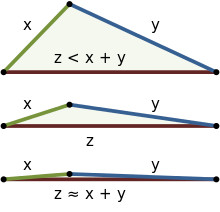
\includegraphics{triangularinequality}
	\end{figure}

We want to show that BFS computes the shortest path $\delta(s,v)$ correctly. We will do it showing first that the distance computed by the BFS procedure bound $\delta(s,v)$ from above.

\begin{theorem}
Suppose we run BFS on a graph $G$ from node $s$ then $v.d \geq \delta(s,v)$. The proof is by induction on the number of \texttt{ENQUEUE} operations. The base case is when only $s$ is in the queue so 
$s.d = 0  = \delta(s,s)$ and $v.d = \infty \geq \delta(s,v)$. Suppose that the hypotesis holds for a number of enqueue operation and in particular that an undiscovered vertex is enqueue from a parent $u$. The inductive hypothesis implies that $u.d \geq \delta(s,u)$. BFS computes the path from $s$ to $v$ composing the path from $s$ to $u$ and adding an edge from $u$ to $v$. this means that: $v.d = u.d +1$
From the theorem \ref{theo:triangular_inequality} follows that $v.d = u.d +1 \geq \delta(s,u) +1 \geq \delta(s,v)$.
\end{theorem}

We have bounded BFS path length from $s$ from above. BFS computes a path which is clearly always less or equal shorter than the shortest possible one. We move on proving that the path it computes are actually the shortest possible so $v.d = \delta(s,v)$.
We now shows that BFS manage in its queue at most two distinct distance values.

\begin{theorem}{\textbf{BFS computes the shortest path from $s$ to all reachable nodes}\hfill \\}
Suppose that for some node (pick up the closest to $s$) $v.d \neq \delta(s,v)$,  then follows that $v.d \geq \delta(s,v)  \wedge \; v.d \neq \delta(s,v) \Rightarrow  v.d > \delta(s,v) $. Let $(u,v)$ an edge then it follows that $\delta(s,v) = \delta(s,u) + 1 = u.d +1$ since $v$ is the first node for which the inequality hold than the BFS path from $s$ to $u$ is the shortest possible\footnote{$\delta(s,u) = u.d$}.
Putting all together we obtain\footnote{$\delta(s,v) = \delta(s,u) + 1 = u.d +1$} 
\[
v.d > u.d + 1 
\]

Consider now the status of $v$ at the time $u$ is explored by BFS procedure. It can be one of the following three cases:
\begin{enumerate}
\item $v$ is UNDISCOVERED: so its distance from $s$ will be $u.d +1 \Rightarrow$ (\textbf{CONTRADICTION)}
\item $v$ was already processed (earlier): $v.d \leq u.d \Rightarrow$ \textbf{(CONTRADITION)}
\item $v$ is DISCOVERED but not PROCESSED: This means that $v$ was discovered when processing a vertex $w$ before $u$ was examined. This also implies that $w$ was processed before $u$ and hence queued before $u$. This implies that $ w.d \leq u.d \Rightarrow w.d+1 \leq u.d +1$. Now, $v$ was discovered by $w$ so its distance from $s$ is $w.d+1$. This allows us to conclude that $v.d \leq u.d+1 \Rightarrow$\textbf{(CONTRADICTION)}.
\end{enumerate}
\end{theorem}

BFS build the so called \textit{Breadth tree} which consist of all the simple (and shortest) paths from $s$ to any reachable (from $s$) vertices \footnote{Those vertices which have a not null parent}. Note that this tree is not unique, and depends on the order in which nodes in the adjacency lists are examined. Node can be discovered using different edges.


\section{Exercices}
%---Problem------------
\begin{problem}
There are two types of professional wrestlers:  babyfaces  ( good guys) and
heels ( bad guys ). Between any pair of professional wrestlers, there may or
may not be a rivalry. Suppose we have n professional wrestlers and we have a list
of r pairs of wrestlers for which there are rivalries. Give an O.n C r/-time algo-
rithm that determines whether it is possible to designate some of the wrestlers as
babyfaces and the remainder as heels such that each rivalry is between a babyface
and a heel. If it is possible to perform such a designation, your algorithm should
produce it.
\begin{solution}
This is a two-color graph coloring problem which is easily solvable in linear time (we are also asking if the graph is bipartite).
We create a node for each professional wrestler and connect them using the relation coded into the $r$ pairs. We then start coloring the graph from a random node and at each level we switch color. If we encounter a node which was previously colored with a different color\footnote{This means that two vertex on a edge that were preivously coloured with different colors are now of the same color.} the such graph is not bipartite and so is not possible to divide \textit{babyfaces} from \textit{heels}. If we consume all the nodes, then the output graph is a proper bipartition.
\end{solution}


\end{problem}



%---Problem------------
\begin{problem}
\textit{Show the d and $\pi$ values that result from running breadth-first search on graph pictured in figure \ref{fig:graphex}, using vertex 3 as the source}.


	\begin{figure}
	\label{fig:graphex}
	\centering
		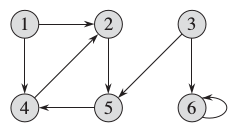
\includegraphics{graphEx}
	\end{figure}
\begin{solution}
\[d(3) = 0 , d(1) = \infty , d(5) = d(6) = 1 , d(4) = 2 ,d(2) = 3\].
\[d(3) = NIL , \pi(1) = NIL , \pi(5) = \pi(6) = 3 , \pi(4) = 5 ,\pi(2) = 4\].
	\end{solution}
\end{problem}


%---Problem------------
\begin{problem}
\textit{Show the d and $\pi$ values that result from running breadth-first search on graph pictured in figure \ref{fig:graphex2}, using vertex 3 as the source}.


	\begin{figure}
	\label{fig:graphex2}
	\centering
		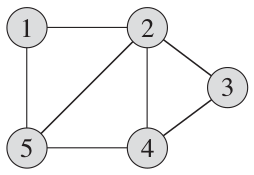
\includegraphics{graphEx2}
	\end{figure}
\begin{solution}
\[d(3) = 0 , d(1) = \infty , d(5) = d(6) = 1 , d(4) = 2 ,d(2) = 3\].
\[d(3) = NIL , \pi(1) = NIL , \pi(5) = \pi(6) = 3 , \pi(4) = 5 ,\pi(2) = 4\].
	\end{solution}
\end{problem}



%---Problem------------
\begin{problem}
The incidence matrix of a directed graph $G=(V,E)$ with s.t. $E$ is a not reflexive relation  is a
$V \times E$ matrix $B = b_{ij}$ such that:
\[
    b_{ij}=\left\{
                \begin{array}{ll}
                  -1 &\text{if j leaves i}\\
                  1 &\text{if j enters i}\\
                  0 &\text{otherwise}
                \end{array}
              \right.
  \]
What the entries of $BB^T$ represents?

	\begin{solution}
	
	\end{solution}
\end{problem}



%---Problem------------
\begin{problem}
\textit{Given an adjacency-list representation of a directed graph, how long does it take
to compute the out-degree of every vertex? How long does it take to compute the
in-degrees?}

	\begin{solution}
\begin{itemize}
\item Out-degree is easy since each node stores the adjacency information as out edges. So out-degree is simply the length of the list which is usually stored as list's attribute hence accessible in $O(1)$. If it 
is the case the time complexity is $O(|V|)$ otherwise we need to inspect all the edges yelding to a $O(|E|)$. 
\item In-degree for node $i$ requires to collect adjacency information from all the other nodes $j \neq i$. Complexity is $O(|E|)$.
\end{itemize}

	\end{solution}
\end{problem}




%---Problem------------
\begin{problem}
\textit{Give an adjacency-list representation for a complete binary tree on 7 vertices. Give
an equivalent adjacency-matrix representation. Assume that vertices are numbered
from 1 to 7 as in a binary heap.}

\begin{solution}

\begin{description}

\item [Adjancency Matrix]\hfill \\
\begin{tabular}{|l|l|l|l|l|l|l|l|}
\hline
\textbf{}  & \textbf{1} & \textbf{2} & \textbf{3} & \textbf{4} & \textbf{5} & \textbf{6} & 7          \\ \hline
\textbf{1} & \textit{0} & \textit{1} & \textit{1} & \textit{0} & \textit{0} & \textit{0} & \textit{0} \\ \hline
\textbf{2} & \textit{0} & \textit{0} & \textit{0} & \textit{1} & \textit{1} & \textit{0} & \textit{0} \\ \hline
\textbf{3} & \textit{0} & \textit{0} & \textit{0} & \textit{0} & \textit{0} & \textit{1} & \textit{1} \\ \hline
\textbf{4} & \textit{0} & \textit{0} & \textit{0} & \textit{0} & \textit{0} & \textit{0} & \textit{0} \\ \hline
\textbf{5} & \textit{0} & \textit{0} & \textit{0} & \textit{0} & \textit{0} & \textit{0} & \textit{0} \\ \hline
\textbf{6} & \textit{0} & \textit{0} & \textit{0} & \textit{0} & \textit{0} & \textit{0} & \textit{0} \\ \hline
\textbf{7} & \textit{0} & \textit{0} & \textit{0} & \textit{0} & \textit{0} & \textit{0} & \textit{0} \\ \hline
\end{tabular}
\hfill \\
\item [Adjancency list] \hfill \\
\begin{verbatim}
1:  2 -> 3 -> NIL
2:  3 -> 4 -> NIL
3:  5 -> 6 -> NIL
4: NIL
5: NIL
6: NIL
7: NIL
\end{verbatim}
\end{description}
\end{solution}
\end{problem}

%---Problem------------
\begin{problem}
The transpose of a directed graph $G = (V,E)$  is the graph $G = (V,E^T)$, where
$ E^T = \{ (v,u) \in V \times V \: : \: (u,v) \in E \}$. Thus $G^T$ is $G$ with all edges reversed.
Describe an efficient algorithm for computing $G^T$ for both  list-matrix adjacency  graph representation. What is the running time complexity of your solutions?

\begin{solution}
\begin{description}
\item [Adjacency List] \hfill \\
The previous algorithms runs in $O(|E|)$. Is thus linear in the number of edges.
	\begin{algorithm}
 \KwData{Graph  $G = (V,E)$}
 \KwResult{graph $G^T = (V,E^T)$}
 $E^T[v.size()] \gets $ initialize adjacency lists\;
 
 \For{$u  \in V$}{
 	 \For{$(u,v) \in E[u] $}{
		 $E^T[v] \gets  (v,u):E^T[v]$\;
  }
  }
 
\Return{$(V,E^T)$}\;
\end{algorithm}



\item [Adjacency Matrix] \hfill \\	
Adjacency matrix for $E^T$ is simply the transpose of $E$. It runs in linear time in the size of matrix which for dense graph is linear in the number of edges in $G$, but for sparse graph is quadratic (yelding so to a quadratic time algorithm).
\end{description}

\end{solution}
\end{problem}

%---Problem------------
\begin{problem}
Given an adjacency-list representation of a multigraph  $G = (V,E)$, describe an
$O(V + E)$ time algorithm to compute the adjacency-list representation of the
“equivalent” undirected graph  $G = (V,E')$, where $E'$ consists of the edges in $E$
with all multiple edges between two vertices replaced by a single edge and with all
self-loops removed.

\begin{solution}
Solution is easy if we use a visiting algorithm which takes care to avoid cycles and visit every nodes of each connected component exaclty once (this implies that whenever two nodes $(u,v)$ are connected by more than once edge we process only one of them, otherwise we would visit $v$ twice, which is contradicts with the the fact that we visit a node only once). This runs in $O(V+E)$.

	\begin{algorithm}
 \KwData{Graph  $G = (V,E)$}
 \KwResult{graph $G^T = (V,E')$}
 $E^T[v.size()] \gets $ initialize adjacency lists\;
 $visited[v.size()] \gets FALSE$\;

 \For{$n  \in V$}{
 	 \If{visited[n] == FALSE}{
		%visit component that starts in n 	 	
 	 		$Q.queue(s)$\;
 	\While{$! Q.empty()$}{
 		$u \gets Q.dequeue()$\;
 		$visited[u] = TRUE$\;
 	  \For{$v  \in E[u]$}{
 	  	\If{visited[v] == FALSE}{
			 $E'[u] \gets  v:E'[u]$\;
		     $E'[v] \gets  u:E'[v]$\; 	  	
 	  	}
 	  }
 	 }
  }
 }
\Return{$(V,E')$}\;
\end{algorithm}


\end{solution}
\end{problem}

%---Problem------------
\begin{problem}
Most graph algorithms that take an adjacency-matrix representation as input re-
quire time $\Omega(V^2)$, but there are some exceptions. Show how to determine whether
a directed graph G contains a universal sink a vertex with $|V|-1$ in-degree and out-degree $0$ in $O(V)$ using adjacency matrix.
\begin{solution}
We compute the sum of all the column of the matrix. Whenever we found a $1$ set the corrensponding row as a not suitable candidate as sink element because its out-degree is at least one.
We then check is there is some column sum which sums up to $|V|-1$ and whose boolean flag is not set to false.

\end{solution}
\end{problem}


%-----END OF CHAPTER GRAPH---------------------------

\chapter{Set}
\section{MultiSet}

\chapter{Associative Array - Dictionary}
\section{Map}
\section{MultiMap}
\section{Hash table - Hash Map}
\iffalse
http://www.tommyds.it/doc/benchmark.html
\fi
\chapter{Tree}

\section{Binary Search Tree}
The search binary tree data structure is capable of suporting both \textit{dictionary} and \textit{priority queue} operation in time proportional to the height of the tree.
Note that in the average case, for randomly constructed tree , the hight is $\Theta(log n)$ but the worst case is bad, since there is always a way to arrange it items s.t. it degrade to a linked list, with height $O(n)$. Self balancing trees ensure that the hight is always logaritmic in the number of nodes (red-black, or AVL tree are two names for such trees).

Let's start stating what is the invariant that makes the binary search tree so powerful. The binary search property always hold for each node of the tree, and all the operations always manintain such property.


\textbf{For each node of the three $x$ then all the nodes in the left subtree rooted at $x.left$ are strictly smaller  then $x.key$ and all the nodes in the right subtree rooted at $x.right$ are greater or equal than $x.key$.
}

	\begin{figure}
	\label{fig:tree_visits}
	\centering
		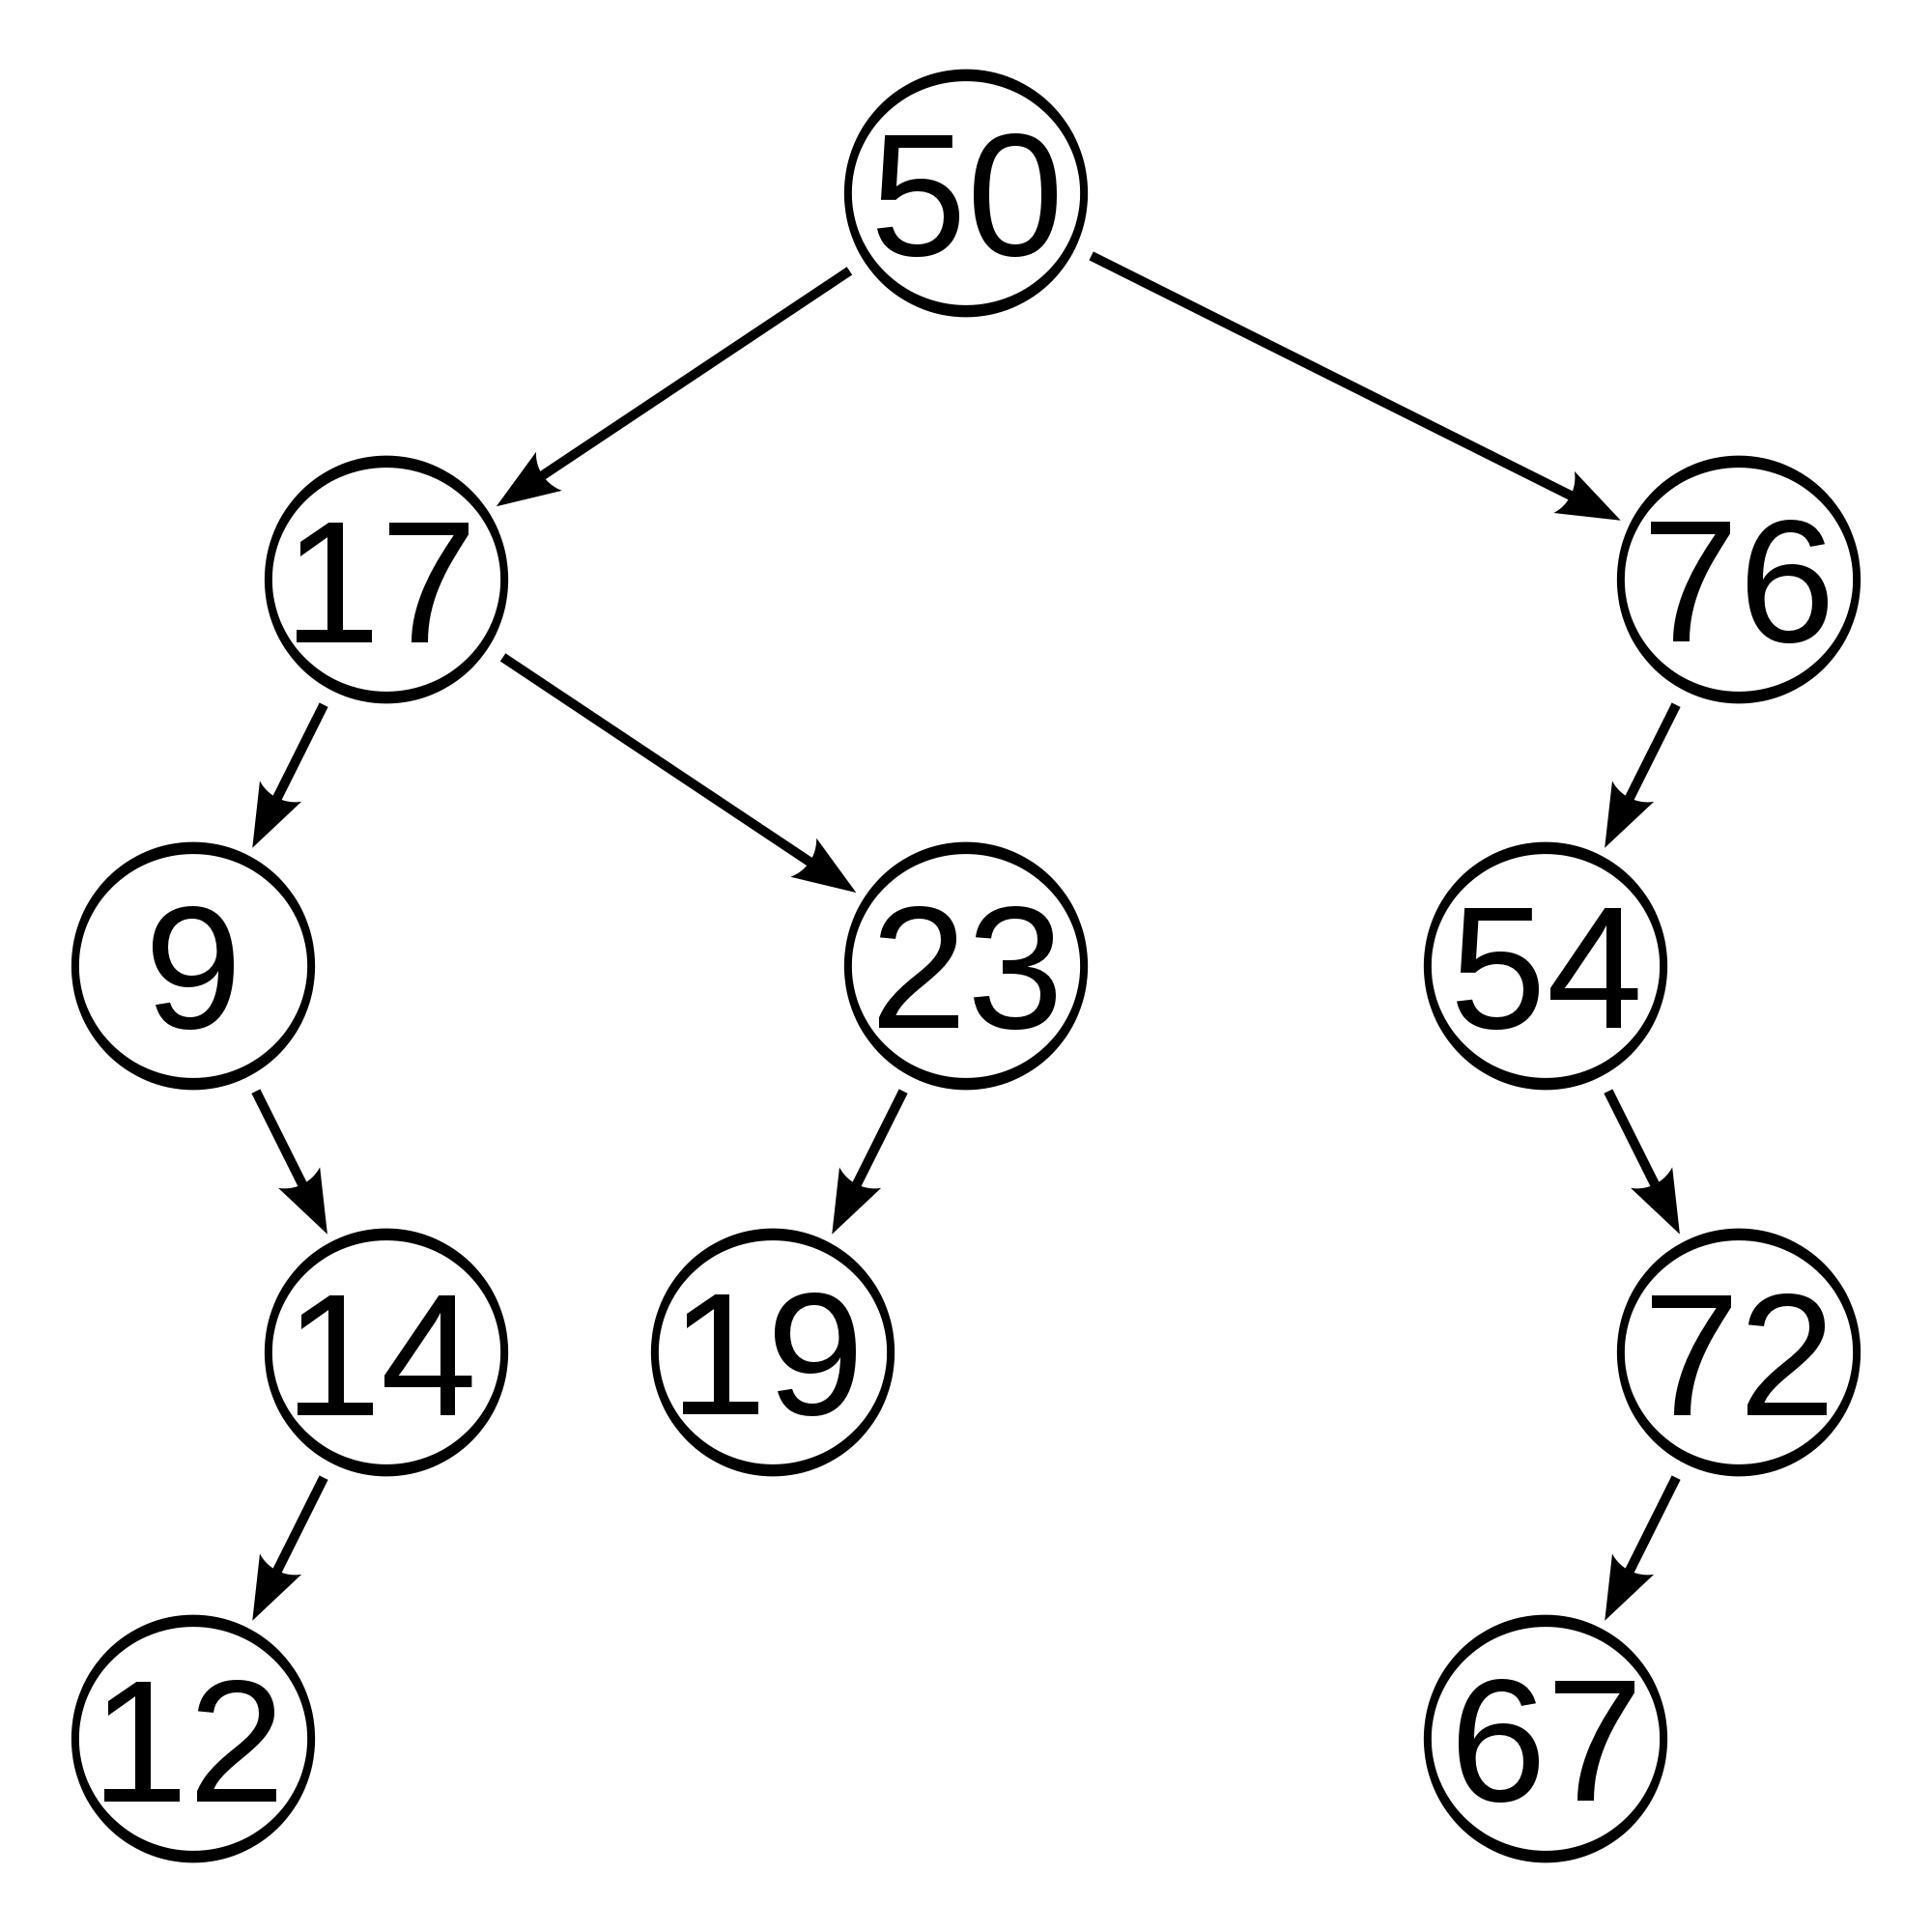
\includegraphics[scale=0.1]{../images/tree_unbl}
		\caption{Binary search tree}
	\end{figure}

It's important to notice the difference between the binary search property and the heap property. The heap property states that for each nodes, the key of the children  of a node $x$ have to be lesser the $x.key$ (both of them). The minimum element is then the root of the tree. Min heap property is less string, and hence easier to mantain, but makes the heap less poweful than the binary search tree. For instance search in a heap costs linear time. Moreover the heap is not able to print out all the element it stores in \textbf{sorted order} in linear time. It takes $\Theta(nlogn)$ since at each min extraction the min heap needs to be restored bubbling up some nodes from the new root to the leaf (in $O(log n)$) 

It is possible to print all the element stored in a search tree in sorted order simply using the so called \textbf{in order} visit of the tree. Given a tree rooted at $x$ is first visit all the nodes of the left subtree, then prints the key of $x$, and finally prints all the nodes in the right subtree.



\begin{algorithm}
\Fn{IN-ORDER(x)}{
		\If{$x=NIL$}{
			\Return \;		
		}	
		$IN-ORDER(x.left)$\;
		$process(x.key)$\;
		$IN-ORDER(x.right)$\;
	}
\caption{In order visi of a binary (search) tree }
\end{algorithm}

Intuitively this works because  the recursion walk down the leftmost path of the tree first reaching the minimum element (which is always a leaf) then prints the that element and recurs on its right subtree if present. Again starting from this node we walk our way down to the leftmost subtree, which in other word is the smallest element among all the greater element of the element just printed out. This is the successor of the printed element! So we alway print an element and its successor.

Changing the order in which we process the node and the recursive calls will make us visit the tree in different order. There are other two ways to arrange the recursive calls and the process the node (see algorithms \ref{alg:pre} and \ref{alg:pst}). 
\begin{itemize}
\item the \textbf{pre-order} visit process the current node first and then recursively visit the left and right subtrees.
\item the \textbf{post-order} visit, as the name suggest processs the current node after processing left and right subtree.
\end{itemize}


\begin{algorithm}
\Fn{PRE-ORDER(x)}{
		\If{$x=NIL$}{
			\Return \;		
		}	
		$process(x.key)$\;
		$IN-ORDER(x.left)$\;
		$IN-ORDER(x.right)$\;
	}
\caption{Pre order visi of a binary (search) tree }\label{alg:pre}
\end{algorithm}


\begin{algorithm}
\Fn{POST-ORDER(x)}{
		\If{$x=NIL$}{
			\Return \;		
		}	
		
		$IN-ORDER(x.left)$\;
		$IN-ORDER(x.right)$\;
		$process(x.key)$\;
	}
\caption{Post order visi of a binary (search) tree }\label{alg:pst}
\end{algorithm}

What is the running time of a such visit on a tree composed of $n$ nodes?
We should start noticing that a visit at least print all the elements once so its running time canno be less than $\Omega(n)$.
Noticing that no nodes is accessed twice gives us that the running time is also $O(n)$. This allows us to conclude that the running time is in reality $\Theta(n)$.

It is important to notice that the visit can also be implemented in a non-recursive procedure. non-recursive calls can be important when the height of the tree is not garanteed to be logaritmic in the number of nodes. Infact when logaritmic the recursive stack of calls has logaritmic length which is not a problem even on tree of a million elements. If the tree ha linear height, on the other hand, this could cause a stack error.

FThe in order walk can be implemented using a stack as an auxiliary data structure that stores the nodes to be processed (taking care of not adding any $NIL$) and whenever we traverse on a $NIL$ subtree we pop from the stack (which contains a valid element), process that element and go right.

\begin{algorithm}
\Fn{IN-ORDER-ITERATIVE(x,S)}{
		$S.push(x)$\;
		$current=x$\;
		\While{$S.size() > 0$}{
			\eIf{$current \neq NIL$}{
			\If{$current.left\neq NIL$}{
					$S.push(current.left)$\;
					
				}
			$current=current.left$
			}{
				$current=S.pop()$\;
				$process(p)$\;
				\If{$current.right \neq NIL$}{
				$S.push(current.right)$\;
				}
				$current=current.right$
			}
		}
		
	}
\caption{In order iterative visit }\label{alg:pst}
\end{algorithm}

The pre-order iterative visit can be implemented using a queue instead of a stack. The root is enqueued and while the queue is not empty we extract an element from the queue and process it straight away. Then we add, if present, left (first) and right children.

\begin{algorithm}
\Fn{PRE-ORDER-ITERATIVE(x,Q)}{
		$Q.push(x)$\;
		\While{$S.size() > 0$}{
			$current=Q.dequeue()$\;
			$process(p)$\;
			\If{$current.left\neq NIL$}{
				$Q.enqueue(current.left)$\;
			}
			\If{$current.right \neq NIL$}{
				$S.push(current.right)$\;
				}
	
			}
		}
\caption{Pre order iterative visit }\label{alg:pre_iter}
\end{algorithm}


\subsection{Searching}
Searching is one of the key operation that BST allows to be performed in $O(h)$. It work by checking for each visited node if the key of that node is the key we are searching for. If yes the search is succesfull and we can return a pointer to that node. If it is not then we can only search \textbf{one} of the two children. Infact if $k$ is the key to be searched and $x$ the current node then if $k > x.key $ we can continue our search on $x$'s right subtree while if $k \leq x.key $ we can continue on its left subtree. It is clear that using this procedure we walk at each iteration of the algorithm one level down till we reach a leaf. Listing \ref{alg:searchrec} and \ref{alg:searchite} are the recursive and iterative search procedures, respectively.

\begin{algorithm}
\Fn{SEARCH-REC(x,k)}{
		\If{$x==NIL$}{
			\Return NIL\;
		}		
		\If{$x.key == k$}
		{
			\Return x\;
		}
		\If{$x.key \leq k$}
		{
			\Return SEARCH-REC($x.left,k$)\;
		}
		\Return SEARCH-REC($x.right,k$)\;
		}			
\caption{BST search recursive.}\label{alg:searchrec}
\end{algorithm}


\begin{algorithm}
\Fn{SEARCH-ITE(root,k)}{
		\While{$root \neq NIL \wedge root.key \neq k$}{
				\If{$root.ket \leq k$}{
					$root=root.left$\;
				}\Else{
					$root=root.right$\;
				}
			}
			\Return $root$;		
		}			
\caption{BST search iterative.}\label{alg:searchite}
\end{algorithm}


\subsection{Minimum and Maximum}
Minimum and maximum are other two operation supported by BST in $O(n)$ time.
Minimum is the element which is smaller than any other element in the structure. Given a node, from the BST property we already know that all the element smaller than it are in its left subtree.
The minimum element is then the leftmost node not having any left child. This translates to: this node has no element smaller than it.
On the other hand the same line of reasoning holds for the \textit{maximum} element. It is the rightmost node not having right child. Listings \ref{alg:minimum} and \ref{alg:maximum} are the procedures for extracting the minimum and the maximum element from a treee rooted at $root$ (assume not to be $NIL$).

\begin{algorithm}
\Fn{MINIMUM(root)}{
		\While{$root.left \neq NIL$}{
					$root=root.left$\;
			}		
			\Return $root$;
		}			
\caption{BST search iterative.}\label{alg:minimum}
\end{algorithm}

\begin{algorithm}
\Fn{MAXIMUM(root)}{
		\While{$root.right \neq NIL$}{
					$root=root.right$\;
			}		
			\Return $root$;
		}			
\caption{BST search iterative.}\label{alg:minimum}
\end{algorithm}

\subsection{Predecessor and Successor}
Successor and predecessor of a node $x$ are defined as the nodes whose key is the next greater and smaller than $x.key$.
By the BST property then it follows that the successor is the element which lies in the right subtree of $x$ (since it is greater). Among all the greater elmenets we should take the smallest one (i.e. the minimum among them). So the successor element is the minimum of the right subtree of $x$. What if the right subtree for $x$ does not exists? The successor must be somewhere in the upper levels,a nd more specifically it must be the first ancestor $x_a$ of $x$ for which $x$ is in \textbf{not} $x_a$'s right subtree( See Figure \ref{fig:bst_successor}). Being in the right subtree of a node $n$ means that out key is greater than the key $n$ (how can a node which its key is smaller than ours be our successor? Its impossible, that is why we look for the first ancestor for which we are in its left subtree, because our key is smaller than its key).
Take for instance the node with key $7$ in figure \ref{fig:bst_successor}. Its successor is node $8$ because if we keep seeking parents points from $7$ at some point we arrive at the point in which the current node is not the right child of a node.

Again fot the simmetry of the BST property the predecessor is the maximum among all the smaller or equal element of $x$. 
Listings \ref{alg:succesor} and \ref{alg:predecessor} are the procedures for extracting the successor and predecessor elements.

	\begin{figure}
	\label{fig:bst_successor}
	\centering
		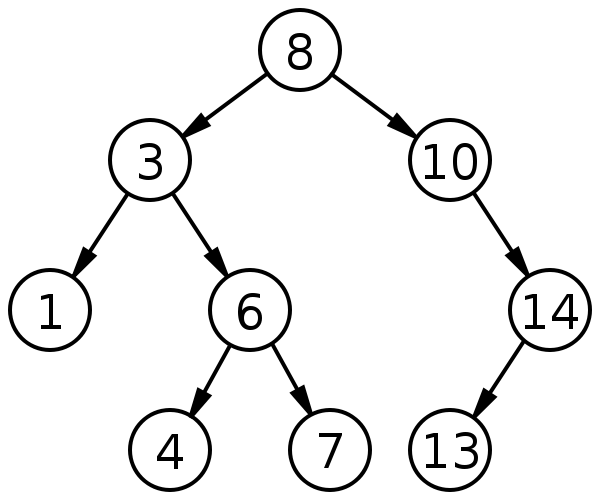
\includegraphics[scale=0.5]{../images/bst_successor}
		\caption{Binary search tree successor and predecessor.}
	\end{figure}
\begin{algorithm}
\Fn{SUCCESSOR(x)}{
		\If{$x \neq NIL \wedge x.right \neq NIL$}{
			\Return $MINIMUM(x.right)$\;
		}
		\While{$p \neq NIL \wedge p.right = x  $}
		{
			$x=p$\;
			$p=x.parent$\;
		}
		\Return $p$\;
		}			
\caption{BST successor procedure.}\label{alg:successor}
\end{algorithm}

\begin{algorithm}
\Fn{PREDECESSOR(x)}{
		\If{$x \neq NIL \wedge x.left \neq NIL$}{
			\Return $MAXIMUM(x.left)$\;
		}
		$p=x.parent$
		\While{$p \neq NIL \wedge p.left = x  $}
		{
			$x=p$\;
			$p=x.parent$\;
		}
		\Return $p$\;
		}			
\caption{BST predecessor procedure.}\label{alg:successor}
\end{algorithm}

\subsection{Insert and Delete}

Insertion and delete are two operation that modifiy the structure of the tree. We should take care of performing them ensuring that the BST property hold at the end of each of these two operation execution on the tree. BST has to be and invariant of these procedures.
As we will see insertion is quite easy to design and implement while the delete operation requires some extra care.
\subsubsection{Insert}
The insertion procedure solves the following problem: given a key $k$ we would like to insert it into the tree rooted at $root$. 
The idea is that we need to search for the right spot where to insert  a newly constructed element which keys is $k$. 
The procedure shown in Listing \ref{alg:insert} outline the ided behind insertion in a BST (See Figure \ref{fig:insertion}).
\begin{algorithm}
\Fn{INSERT(root,z)}{
			\If{$root==NIL$}{
				$root=z$\;
				\Return \;			
			}
			$y=root$\;
			\While{$y \neq NIL$}{
				\If{$y.key \geq z.key$}{$y=y.left$\;}
				\If{$y.key < z.key$}{$y=y.right$\;}
			}
			$z.parent=y$\;
			\If{$y.key \geq z.key$}{$y.left=z$\;}
			\Else{$y.right=z$\;}
			
}
\caption{Iterative BST insert procedure.}\label{alg:insert}
\end{algorithm}

\begin{figure}
	\label{fig:insertion}
	\centering
		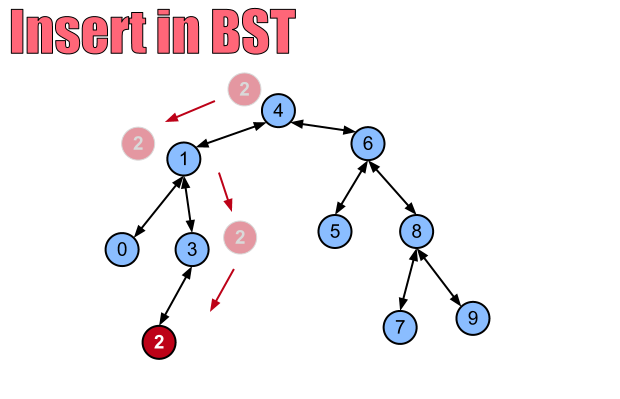
\includegraphics[scale=0.7]{../images/bstinsert}
		\caption{Inserting a node with key $2$ in a BST.}
	\end{figure}

We navigate the BST from the root to the leafs and we stop as soon we found a $NIL$ spot which is good for inserting the element $z$ (good means that preserves the BST property).
Let's call this element $y$. We need to set $z$'s parent pointer to $y$ and make $z$ child of $y$ by updating the correcnt $y$ child pointer.

\begin{algorithm}
\Fn{INSERT(root,c,p,z)}{
			\If{$p == NIL$}{
				$root=z$\;
				\Return \;
			}
			$side=NIL$\;	
			\If{$c == NIL$}{
				$z.p=p$\;
				
			\If{$z.key \leq p.key$}{				
				$p.left=z$\;
			}\Else{
				$p.right=z$\;			
			}
			
			}\Else{
				\If{$z.key \leq p.key$}{				
				$INSERT(root,c.left,c)$\;
			}\Else{
				$INSERT(root,c.right,c)$\;
			}
			}
			
	}
\caption{Recursive BST insert procedure.}\label{alg:insert}
\end{algorithm}


\subsubsection{Delete}
Delete operation is a bit more delicate and requires some extra care. Let's note that deleting a node with no children at all is an easy case since it is a leaf. Deleting a leaf does not ruin the BST property.
For instance take the node $13$ in figure \ref{fig:bst_successor}. Deleting it leaves the tree withouth doing any further operations preserves the BST property. Another easy case is when the node has only one child (the node $10$ or $14$ in figurer \ref{fig:bst_successor} for instance).  What we need to do is to delete that node and move the only one substree (right or left, in its entirety) up one level to the just deleted node parent node. 
Let's say for instance that we are about to delete node $10$. What we have to do is to set $8$'s right child pointer to node $14$ and to update $14$'s parent pointer such it points to node $8$. In other words we elevate the only present child   to the position of the to be deleted node ($z$) by modifying $z$'parent ($8$  in this case).

If $z$ has both children then we can't simply delete the node because this would leave an hole in the data structure, and consequently, some nodes would be unreachable. For instance imagine we are about to delete node number $6$ in Figure \ref{fig:bst_successor}. Deleting that node would leave nodes $4$ and $7$ unlinked and unreachable from the root!
We need to substitute $z=6$ with some other node. Which one? The only node which can be substituted to $z$ and still satisfies the BST is $z$ successor because all nodes at $z$'s left subtree would still be lesser or equal than $z$'s successor and all element on $z$'s right subtree would be still greater than $z$ successor (which will not belong to $z$ subtree any more and was smaller than all element in $z$ right subtree, being the minimum among them!).
If $z's$ successor ($y$) is $z$'s right child then we simply substitute $z$ by $y$. 
If is not then we need to make $y$ right subtree (the only one present since it's $z$'s  successor) left child of $y$ parent (which cannot be  $z$!) and then move $y$ in place of $z$.


As and example take the node $6$ in Figure \ref{fig:insertion}. If we substitute $6$ by $7$, its successor, then the BST property is still satisfied since $5$ is still less than $7$ and $8$ and $9$ are greater than $7$.

\begin{figure}
	\label{fig:insertion}
	\centering
		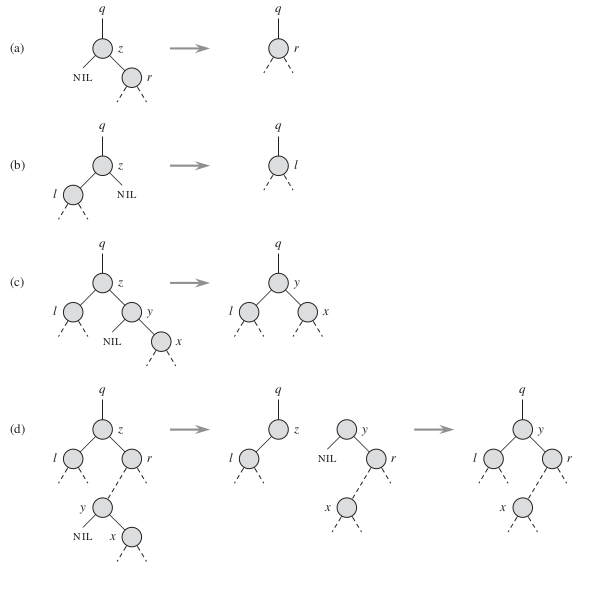
\includegraphics[scale=0.7]{../images/bstdelete}
\caption{Deleting a node $z$ from a BST. case \textbf{(a)} deals with the case $z$ has not left child. Its right child (which may be NIL, and if it is, this handle the case where both children are NIL) is substituted to $z$. Case \textbf{(b)} is when $z$ has only left subtree, in this case again we simply substitute $z$ by $z$'s left child. Case \textbf{(c)} is when $z$ has both children  but is successor is $z$ right child! In this case we simply elevate $y$ at $z$ place without modifying the structures of any node at lower levels. Case \textbf{(d)} deals with the case when $z$ successor is not $z$'s right child. 
If this is the case then we can't simply move $y$ in place of $z$ since $y$ may carries a whole subtree (right one) with it. We need to move $y$ right subtree in place of $y$ first and then safely move $y$ in place of $z$. }
	\end{figure}

Since we are moving subtree around it is useful to write a utility procedure that takes a tree and two subtree rooted at $u$ and $v$ respectively. Goal of this procedure is to substitute $u$ with $v$ making sure that parent links are correctly set.

\begin{algorithm}
\Fn{TRANSPLANT(root,u,v)}{
			\If{$u==NIL$}{
				$root=v$\;
				\Return \;			
			}
			\If{$u.p.left==u$}{
				$u.p.left=v$\;
			}\Else			
			{
				$u.p.right=v$\;
			}
			\If{$v \neq NIL$}{
				$v.p = u.p$\;			
			}
}
\caption{TRANSPLANT procedure. It takes two subtree rooted at $u$ and $v$ and substitue $u$ with $v$ making sure that parent links are preserved.}\label{alg:transpant}
\end{algorithm}

Using precedure \ref{alg:transpant} it is not hard to write a procedure for deleting a node into a BST.
\begin{algorithm}
\Fn{DELETE(root,z)}{
			\If{$Z.left==NIL$}{
				$TRANSPLANT(root,z,z,right)$\;
				\Return \;			
			}
			\If{$Z.right==NIL$}{
				$TRANSPLANT(root,z,z,left)$\;
				\Return \;
			}
			$y=SUCCESSOR(root,z)$\;
			\If{$y \neq z.right$}{
					$TRANSPLANT(root, y, y.right)$\;
					$y.right=z.right$\;
					$y.right.p=y$\;
			}
			$TRANSPLANT(root,z,y)$\;
			$y.left=z.left$\;
			$y.left.p=y$\;
			
		
}
\caption{Delete procedure. The four possible cases are handled.  Note in particlar how the case where $z$ has both children is handled. We first find its successor $y$ (node with the  smallest in its (NOT NIL) right subtree. Since we want to move $y$ from its original location and put in place of $z$. Now if $y$ is $z$'s right child then we first move $y$ right subtree in plce of $y$. We do so by updating $y$'s parent (inside transplant procedure) and updating $x$ parent pointer  to points to $y$ parent $r$. We subsequentially change $y$ right child pointer to point to $z$ right child. We can safely move $y$ into place of $z$. We do so by transplanting $y$ into $z$We do so updating $z$'s parent pointer (inside transpant operation) and then updating $z$ left child to point to its new parent $y$.}\label{alg:transpant}
\end{algorithm}

Complexity of DELETE procedure is linear in the height of the tree. All operations performed are constant time but successor which is $O(h)$.

\section{Self Balancing Tree}
\subsection{B Tree}
\subsection{B+ Tree}

\subsection{Adelson-Velsky Landis Tree - AVL Tree}
\subsection{Red Black Tree}
\subsection{Splay Tree}


\section{Space-partitioning trees}
\subsection{Kd Tree}
\subsection{R Tree}
%\chapter{Dynamic Programming}
Transforming complex problems into a sequence of subproblems whose solutions can be used to construct a solution for the bigger and original problem.
It also is a general framework for analyzing and solving optimization problems effectively and fast\footnote{Usually optimization problems require exponential time to be solved.}.

Dynamic programming decompose large problem in a collection of small problems which can be solved in linear order (forming a implicit conceptual DAG) one after the other, from the \textit{smallest} to the \textit{largest} and using solution to the small ones to solve the bigger ones. 

\section{DAG shortest Path}
Probably one of the easiest example that can depict the concept behind DP is the problem of computing the shortest path in a DAG (because of the analogy with DP itself which linearize problems and the fact that DAGs can be linearized s.t. all the edges point forward).

\begin{framed}
A DAG is a graph such that exists a topological ordering (see figure \ref{fig:DAGsort}) of nodes $v1,v2, \ldots,v_n$ (we assign an differen interger to each  node) s.t. for each edge $(i,j)$ we have that $i<j$.
	
\end{framed}

	\begin{figure}
	\label{fig:DAGsort}
	\centering
	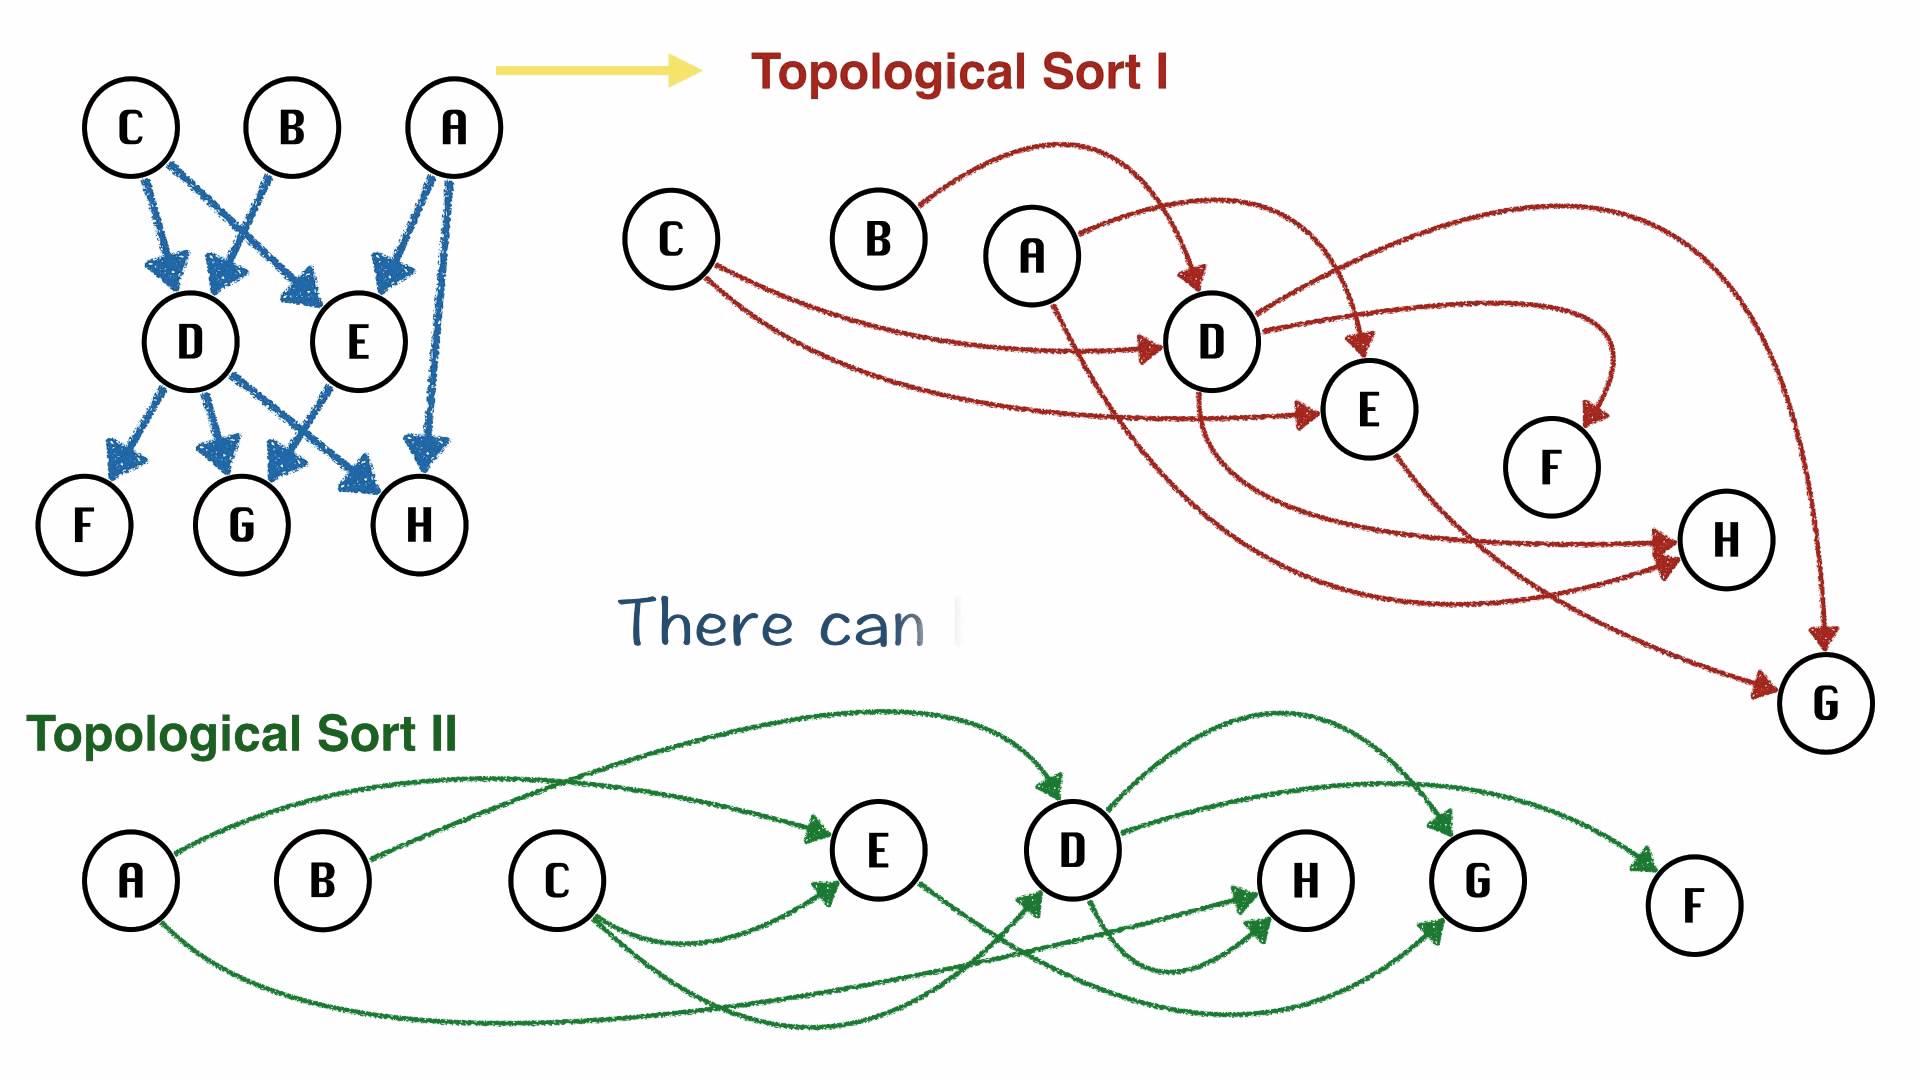
\includegraphics[width=\textwidth]{../images/DAGsort}
	\caption{DAG topological sorting}
	\end{figure}


Problem here is to find the shortest (largest works fine as well) between a two nodes $s$ called source and $d$ destination.
Consider, the DAG in figure \ref{fig:dagexample} with $s=A$ and $d=E$
	\begin{figure}
	\label{fig:dagexample}
	\centering
	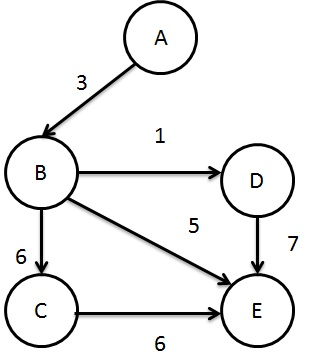
\includegraphics[width=0.5\textwidth]{../images/dagexample}
	\caption{DAG topological sorting}
	\end{figure}
In order to compute the shotest path it is usefult to think as follows. We know that any possible path that leads to $E$ eventually has to go through ieither $C,B,D$ cause those are the only edges that point inwards to $E$, out destination.
Is like willing to go to Rome which has three roads only  from outside the city to the center.
The length of the shortest path is clearly the following:
\[
	dist(A,E) = min\{dist(A,D)+weigth(D,E), dist(A,C)+weigth(C,E), dist(A,B)+weigth(B,E)\}
\]
As one can see from the above expression this formulation is made up of 3 smaller subproblems which can be solved the same way as the bigger problem.
One can ask the question, how much does the shortest path between $A$ and $D$ weights? Well it is formulaed the same way (ansering the question, how many inward edges $D$ has?):
\[
dist(A,D) = min\{dist(A,B) + weight(B,D)\} = dist(A,B) + weight(B,D)
\]
The nice thing about this approach is that if we work our way from A to E in a left to right manner (assuming DAG topological order) at time of computing any \textit{dist} subproblem we already have computed all relevant subproblems that allow us to solve the particular istance at hand (proceeding this way until we have solved all the subproblems).
A simple schematization of this ideas lead us to the pseudocode in listing (\ref{alg:dagshortest})
\begin{algorithm}\label{alg:dagshortest}
\Fn{DAG\_SHORTEST (A,E)}{
	\For{$i \gets 1$ \textbf{to} $n$} {
		$dist(A,n) \gets \infty$;
	}
	$dist(A,A) \gets 0$;\\
	\For{$v \in V \setminus\{A\}$ \texttt{in linearized order} }{
		$dist(A,v) \gets \min_{(u,v) \in E}{dist(A,u) + weight(u,v)}$
	}
}
\caption{DAG shortest path algorithm}
\end{algorithm}
Start at the very right. Distance from source to source is obviously zero, you don't need to move at all. 
Next node taken in consideration is (because they are linearly ordered) is $B$ for which the only edge having it as second node is $(A,B)$. Shortest path to 
$B$ is then $dista(A,A)=0 + weight(A,B) =3$ which totals $3$. Next ones is $C$ which has only one edge leading into it, $(B,C)$. $dist(A,C) = dist(A,B) + weight(B,C) = 3+6=9$.
Next one is $D$, again only one edge leading into it, $(B,D)$ which allows us to compute its shortest path from A: $dist(A,D) = dist(A,B) + weight(B,D) = 3 +1 =4$.
Next one is $E$ our destination node which has the following inwards edges $\{(D,E),(B,E), (C,E)\}$.Shortest path from $a$ to $E$ is then 
the minimum among the following quantities:
\[
	dist(A,B) + weight(B,E) = 3+5=8
\]
\[
	dist(A,C) + weight(C,E) = 7 + 9 = 16
\]
\[
	dist(A,D) + weight(D,E) = 2 +7 =9
\]
Minimum among $5,13,9$ is $5$ which happens to be the shortest path weight between $A$ and $E$ in graph in figure \ref{fig:dagexample}.
Is important to note here that we haven't find the actual \textit{path} but rather the weith of one of the possible shortest path! In order to find the shortest path we need to do some more work and record at each step i.e. at each subproblem solved or in other words when we find an intermediate shortest path value which is the parent node for which happen that the distance is minimal (Among all the inwards edges which one leads to the minimum weight?).
We will record all this informations in an associative array, \textit{parent}:
In the previous example when solving $dist(A,B)$ we found out that the shortest path was hopping through node $A$:  parent[B] = A;
For node $C$ shortest path was going through node B so parent[C] =B;
For node $D$ shortest path was going through node B so parent[D] =B;
For node $B$ shortest path was going through node B so parent[E] =B;
We can work the path backwards from the destination node and reconstruct all the hops using the \textit{parent} relationship.
$path(A,E) = E \rightarrow parent(E) \rightarrow  parent[parent[E]] \rightarrow  \ldots \rightarrow $ until we reach the souce node.

\section{Longest Increasing Subsequence}
The longest increasing subsequence is the problem of finding a subset $V_a=v_{a_1} \leq v_{a_2} \leq\ldots \leq v_{a_k}$, $a_1 < a_2 < \ldots < a_k$ and not other subsequence $V_b=v_{b_1}\leq v_{b_2}\leq \ldots \leq v_{b_l}$, $b_1 < b_2 < \ldots < b_l$ s.t. l > k.

The solution to this problems has to be a sequence of any size of element of the original collection s.t. the its overlall sum is \textbf{maximal}.

The naive approach leads to a $\Theta(2^n)$ algorithm which considers possible subset. Since there are an exponential number of such subsets this leads to a \textbf{exponential algorithm}.
We can do much better using DP.
Our goal is to recursively formulate the solution in terms of smaller problems than have no dependencies at all with the bigger ones.  Using the DAG analogy this means that for each subproblem to be solved the only information needed are solution to even smaller subproblems.

Let's work our way from the end of the array. What we know for sure is that the last element of the array can't be itself the first of a subsequence longer than one.
What we know about the second last element?
If a subsequence starts at this location then its lenght may be one or two depending weather this element is greater or less then the last one.
What about the third last? Again any subsequence starting at this location may be of lengths $1,2,3$ depeding weather it is greater than both the subsequent ones or only of one of them (no matter which one) or lesser than both.
This lead us to the following statement. Working our way backwards, at each location $i$ the longest subsequence starting at $i$ is the longest subsequence starting at any index greater than $i$ s.t. $V[j] > V[i]$ , $j>i$ i.e. the next element must be greater than the element at index $i$ (after all we are trying to find an increasing subsequence). 
Generalizing this idea we can formulate the solution as follows:
\[
LS(n) = 1+ \underset{ \underset{ V[i] > V[n]}{i > n} }{\max}{ LS[i]}
\]
 
In order to solve this problems we have created a list of subproblems with the following properties:
Problems are orderable and there exists a dependence between bigger and smaller problems. Bigger problems depends only on smaller problems, smaller problems depends on even smaller problems and so on until we reach the base case for which we already know the answer or we can compute it withoth using any other subproblem at all.
Each subproblem requires is dependent not only on one (smaller) subproblem but on all the smaller subproblems (the max operator iterate all subproblems till the base case)!
The complexity of solving one subproblem is then the complexity of finding the maximum value in a collection of values which can be done in $O(n)$. since we have to solve $n$ of this subproblems the complexity is quadratic $O(n^2)$. It is important to note that the max operator takes linear time \textbf{only} is we remember the solution to the smaller problems without recomputing them all the times they are required to be solved. This \textit{remembrance} is called \textbf{memoization} and is a key concept in \textbf{dymanic programming}. \textbf{Solution to problems that are required to be solved over and over have to be memoized}. 
Problems that exposes this pattern of decomposition i.e. that requires subproblems to be solved over and over again are said to have the property of \textbf{overlapping subproblems}. Memoization skyrocket the algorithm when a problem has this property.
The following is the pseudocode for the \textit{longest increasing subsequence}.



%\chapter{Glassdoor Google Interview}
%---Problem---------------------------------
\begin{problem}
Suppose that you have a sorted array of integers (positive or negative). You want to apply a function of the form $f(x) = a * x^2 + b * x + c$ to each element x of the array such that the resulting array is still sorted. Implement this in Java or C++. The input are the initial sorted array and the function parameters (a, b and c). 
\end{problem}	

\begin{solution}



\end{solution}	
%\chapter{Project Euler}
\chapterimage{ch4.jpg} % Table of contents heading image
\begin{problem}
If we list all the natural numbers below 10 that are multiples of 3 or 5, we get 3, 5, 6 and 9. The sum of these multiples is 23.
Find the sum of all the multiples of 3 or 5 below 1000.
 \end{problem}
 
 \begin{solution}

\begin{lstlisting}[language=Haskell, caption="Haskell"]
	problem1' = sum . 
	            filter (\x -> x `mod` 3==0 || x `mod` 5 ==0)
\end{lstlisting}


\begin{lstlisting}[language=Matlab, caption="Matlab"]
function sum=problem1(n1,n2,n)
	sum=0;
	 i=1;
     for  i= 1: n-1  
         if or(mod(i,n1) ==0, mod(i,n2)==0)
             sum=sum+i;
         end
	    i=i ++;
end   
\end{lstlisting}                         

\begin{lstlisting}[language=Java, caption="Java"]
                         

public class Problem1 {

	public static void main(String[] args) {
		naiveSolution();	
		alternativeSolution();
	}	
	private static void naiveSolution() {
		int sum=0;
		for(int i=3;i<1000;i++){
			if(i%3==0 || i%5==0)
				sum+=i;
		}
		System.out.println("The sum is " +sum);		
	}
	
	private static  void alternativeSolution() {
		//multiple of 3 are of type 3*k with 3*k<1000
		//multiple of 5 are of type 5*k with 5*k<1000
		//sum up all the multiple of 3 and 5 but taking care of subtracting once
		//the multiple of 3 and 5 (15*k) that have been summed twice
	  int sum= 3*sumFirstNNumber(333)+5*sumFirstNNumber(199)-15*sumFirstNNumber(66);
	  System.out.println("The sum is " +sum);	
	}
	
	private static int sumFirstNNumber(int n) {
		return (n*(n+1))/2;
	}
\end{lstlisting}

\end{solution}

\begin{problem}
Each new term in the Fibonacci sequence is generated by adding the previous two terms. By starting with 1 and 2, the first 10 terms will be:

1, 2, 3, 5, 8, 13, 21, 34, 55, 89, ...

By considering the terms in the Fibonacci sequence whose values do not exceed four million, find the sum of the even-valued terms.
\end{problem}	
	\begin{solution}

		\begin{lstlisting}[language=Matlab, caption="Matlab"]
function sum=problem2
	S=0;
	i=0;
	j=2;
	sum=2; 
	while (S < 4000000)
	            sum= sum+S
	             S=4*j+i;
	             i=j;
	             j=S;
	end	
            
\end{lstlisting}  

	\end{solution}	
	


\begin{problem}
The prime factors of 13195 are 5, 7, 13 and 29.
What is the largest prime factor of the number 600851475143 ?
\end{problem}	
	\begin{solution}

		\begin{lstlisting}[language=Haskell, caption="Haskell"]
	module Problem3 (problem) where


testInt = 600851475143

problem = last $ problem3 testInt 3 [] 

problem3 :: Integer -> Integer -> [Integer] -> [Integer]
problem3 n a acc
	 |product acc == n =  acc 
	 |n `mod` a==0 = a:problem3 (div n a) (a) acc
	 |otherwise    =problem3 n (a+1) acc
        
\end{lstlisting}  


		\begin{lstlisting}[language=Matlab, caption="Matlab"]
	
function p=problem3(n)
	% the algorithm is based on the fundamental theorem of arithmetic 
	% p will be the largest prime factor of the number n 
	m=n;
	p=0;
	oldp=2;
	while (oldp*oldp <= m )
	         if (mod(m,oldp)==0)
	         	m=m/oldp;
	         	p=oldp;
	         else 
	         	oldp ++;
	         end
	   end
	   if (m > p )
	      p=m;
	    end 
        
\end{lstlisting}  

	\end{solution}	



%---Problem---------------------------------
\begin{problem}
The sum of the squares of the first ten natural numbers is, $12 + 22 + ... + 102 = 385$
The square of the sum of the first ten natural numbers is, $(1 + 2 + ... + 10)2 = 552 = 3025$
Hence the difference between the sum of the squares of the first ten natural numbers and the square of the sum is 3025 - 385 = 2640.
\textbf{Find the difference between the sum of the squares of the first one hundred natural numbers and the square of the sum.}
\end{problem}	

\begin{solution}

		\begin{lstlisting}[language=Haskell, caption="Haskell"]
module Problem6 where

n = 100
problem6 = squareSum - sumSquare
--sum of the first n number = (n^2+n)/2 -> simply becomes squareSum
squareSum = 1/4*(n^4+2*n^3+n^2)
--first create a list with squares of the first n numbers the sum them up
sumSquare = sum $ map (^2) [1..n]
        

		\end{lstlisting}  

\end{solution}	
%------------------------------------------------



%---Problem---------------------------------
\begin{problem}
By listing the first six prime numbers: $2, 3, 5, 7, 11, 13$, we can see that the 6th prime is 13.
\textbf{What is the $10001^{st}$ prime number?}
\end{problem}	

\begin{solution}

		\begin{lstlisting}[language=Haskell, caption="Haskell"]
        
module Problem7 where

limit=10001
--params : last prime, position of the last prime (the nth), current
problem7 :: Integer -> Integer -> Integer -> Integer
problem7 p 10001 _ =  p
problem7 p k c     
    |isPrime c = problem7 c (k+1) (c+2)
    |otherwise = problem7 p k (c+2)
                 
isPrime :: Integer -> Bool
isPrime n = 0 ==  length (dropWhile (\v -> (n`mod`v) /=0) [2..(floor $ sqrt(fromInteger n))])


		\end{lstlisting}  

\end{solution}	
%------------------------------------------------


%---Problem---------------------------------
\begin{problem}

\end{problem}	

\begin{solution}

		\begin{lstlisting}[language=Haskell, caption="Haskell"]
        

		\end{lstlisting}  

\end{solution}	
%------------------------------------------------




%---Problem---------------------------------
\begin{problem}
The four adjacent digits in the $1000$-digit number that have the greatest product are $9 \times 9 \times 8 \times 9 = 5832$.

\begin{multline*}\\
73167176531330624919225119674426574742355349194934\\
96983520312774506326239578318016984801869478851843\\
85861560789112949495459501737958331952853208805511\\
12540698747158523863050715693290963295227443043557\\
66896648950445244523161731856403098711121722383113\\
62229893423380308135336276614282806444486645238749\\
30358907296290491560440772390713810515859307960866\\
70172427121883998797908792274921901699720888093776\\
65727333001053367881220235421809751254540594752243\\
52584907711670556013604839586446706324415722155397\\
53697817977846174064955149290862569321978468622482\\
83972241375657056057490261407972968652414535100474\\
82166370484403199890008895243450658541227588666881\\
16427171479924442928230863465674813919123162824586\\
17866458359124566529476545682848912883142607690042\\
24219022671055626321111109370544217506941658960408\\
07198403850962455444362981230987879927244284909188\\
84580156166097919133875499200524063689912560717606\\
05886116467109405077541002256983155200055935729725\\
71636269561882670428252483600823257530420752963450\\
\end{multline*}
\textbf{Find the thirteen adjacent digits in the $1000$-digit number that have the greatest product. What is the value of this product?}
\end{problem}	

\begin{solution}

		\begin{lstlisting}[language=Haskell, caption="Haskell"]
{-
Naive solution. It simply scan all possible 13tuple of numbers and look for maximum (product of digits)
A more efficient solution could be to consider that a zero cause 13 tuple to have 0 product!
-}
import Data.Char

numberInOneLine :: String -> String
numberInOneLine  = foldl (++) [] . words

splitNumber :: String -> [Integer] -> Integer -> Integer
splitNumber  [] _ v = v 
splitNumber cc@(c:cs) yy@(y:ys) v 
  | v < productNew = splitNumber cs tokenNew productNew 
  | otherwise = splitNumber cs tokenNew v                          
  where
    tokenNew   = (ys++ ([toInteger (digitToInt c)]))
    productNew = product tokenNew 
    productOld = product yy
              
digitize :: Integer -> [Integer]
digitize x
	| x `div` 10 == 0 = [x]
	| otherwise = digitize (x `div` 10) ++ [x `mod` 10]
	

main = do 
  putStrLn "Please Insert the filename where bigNumber is stored:"
  fileName <- getLine
  strRaw <-  readFile fileName 
  let str= numberInOneLine strRaw
  let first13= (digitize (read (take 13 str)))
  let splitted = splitNumber (drop 13 str)  first13 (product first13) 
  putStrLn $ show  (splitted)
  putStrLn $ show  (product first13)        

		\end{lstlisting}  

\end{solution}	
%------------------------------------------------





%---Problem---------------------------------
\begin{problem}
In the $20\times20$ grid below, four numbers along a diagonal line have been marked in red.
\begin{multline*}\\
08\;02\;22\;97\;38\;15\;00\;40\;00\;75\;04\;05\;07\;78\;52\;12\;50\;77\;91\;08\\
49\;49\;99\;40\;17\;81\;18\;57\;60\;87\;17\;40\;98\;43\;69\;48\;04\;56\;62\;00\\
81\;49\;31\;73\;55\;79\;14\;29\;93\;71\;40\;67\;53\;88\;30\;03\;49\;13\;36\;65\\
52\;70\;95\;23\;04\;60\;11\;42\;69\;24\;68\;56\;01\;32\;56\;71\;37\;02\;36\;91\\
22\;31\;16\;71\;51\;67\;63\;89\;41\;92\;36\;54\;22\;40\;40\;28\;66\;33\;13\;80\\
24\;47\;32\;60\;99\;03\;45\;02\;44\;75\;33\;53\;78\;36\;84\;20\;35\;17\;12\;50\\
32\;98\;81\;28\;64\;23\;67\;10\;\begingroup\color{red}26\endgroup\;38\;40\;67\;59\;54\;70\;66\;18\;38\;64\;70\\
67\;26\;20\;68\;02\;62\;12\;20\;95\;\begingroup\color{red}63\endgroup\;94\;39\;63\;08\;40\;91\;66\;49\;94\;21\\
24\;55\;58\;05\;66\;73\;99\;26\;97\;17\;\begingroup\color{red}78\endgroup\;78\;96\;83\;14\;88\;34\;89\;63\;72\\
21\;36\;23\;09\;75\;00\;76\;44\;20\;45\;35\;\begingroup\color{red}14\endgroup\;00\;61\;33\;97\;34\;31\;33\;95\\
78\;17\;53\;28\;22\;75\;31\;67\;15\;94\;03\;80\;04\;62\;16\;14\;09\;53\;56\;92\\
16\;39\;05\;42\;96\;35\;31\;47\;55\;58\;88\;24\;00\;17\;54\;24\;36\;29\;85\;57\\
86\;56\;00\;48\;35\;71\;89\;07\;05\;44\;44\;37\;44\;60\;21\;58\;51\;54\;17\;58\\
19\;80\;81\;68\;05\;94\;47\;69\;28\;73\;92\;13\;86\;52\;17\;77\;04\;89\;55\;40\\
04\;52\;08\;83\;97\;35\;99\;16\;07\;97\;57\;32\;16\;26\;26\;79\;33\;27\;98\;66\\
88\;36\;68\;87\;57\;62\;20\;72\;03\;46\;33\;67\;46\;55\;12\;32\;63\;93\;53\;69\\
04\;42\;16\;73\;38\;25\;39\;11\;24\;94\;72\;18\;08\;46\;29\;32\;40\;62\;76\;36\\
20\;69\;36\;41\;72\;30\;23\;88\;34\;62\;99\;69\;82\;67\;59\;85\;74\;04\;36\;16\\
20\;73\;35\;29\;78\;31\;90\;01\;74\;31\;49\;71\;48\;86\;81\;16\;23\;57\;05\;54\\
01\;70\;54\;71\;83\;51\;54\;69\;16\;92\;33\;48\;61\;43\;52\;01\;89\;19\;67\;48\\
\end{multline*}
The product of these numbers is $26 \times 63 \times 78 \times 14 = 1788696$.

\textbf{What is the greatest product of four adjacent numbers in the same direction (up, down, left, right, or diagonally) in the $20\times20$ grid?}

\end{problem}	

\begin{solution}

		\begin{lstlisting}[language=Java, caption="Java"]
        
package euler;

import java.io.IOException;
import java.nio.file.FileSystems;
import java.nio.file.Files;
import java.nio.file.Path;



public class Problem11BruteForce {
	public static int size=4;
	public static long maxPossibleValue=multiplicateKtimes(99,size);

	public static long getProductElmts(int[][] matrix, int i, int j, int inci, int incj){
		/**
		 * return the product of the tuple of *size element* starting at i,j in the direction of the vector (inci,incj)
		 * **/
		long product =1;
		for(int k=0;k<size;k++){
			int val= matrix[i+k*inci][j+k*incj];
			product*=val;
		}
		return product;
	}

	private static long multiplicateKtimes(int num, int size2) {
		long res=1;
		for(int i=0;i<size2;i++)
			res*=num;	

		return res;
	}

	/*
	 * There is no need to check all the 8 directions-> 4 are enough
	 * Return as soon I get (if happen) the max possible value = 99^size
	 * */
	public static long findMaxProduct(int[][] matrix){
		int m = matrix.length;
		int n = matrix[0].length;
		long max =Long.MIN_VALUE;
		for(int i = 0; i < m; i++){
			for (int j = 0; j < n; j++) {
				//horizontal right
				long prodHor=0, vertDown=0, diagR=0,diagLeft=0;
				if(j<n-size)
					prodHor=getProductElmts(matrix, i, j, 0, 1);

				//verticalDown 
				if(i<n-size)
					vertDown=getProductElmts(matrix, i, j, 1, 0);

				//diagonal  right
				if(j<n-size-1 && i<n-size-1)
					diagR=getProductElmts(matrix, i, j, 1, 1);

				//diagonal  left
				if(j>size-1 && i<n-size-1)
					diagLeft=getProductElmts(matrix, i, j, 1, -1);

				max=Math.max(max,Math.max(diagLeft,Math.max(diagR,Math.max(prodHor, vertDown))));
				
				if(max>=maxPossibleValue){
					return max;
				}

			}
		}
		return max;
	}

	public static int [][] readMatrix(String spath){
		Path path = FileSystems.getDefault().getPath(spath, "matrix");
		try {
			String fileContent= new String(Files.readAllBytes(path));
			int[][] matrix= new int [20][20];
			String[] lines = fileContent.split("\n");
			for(int i=0;i<lines.length;i++){
				String[] lineSplitted = lines[i].split(" ");
				for(int j=0;j<lineSplitted.length;j++){
					matrix[i][j] = (Integer.parseInt(lineSplitted[j]));
				}
			}
			return matrix;


		} catch (IOException e) {
			// TODO Auto-generated catch block
			e.printStackTrace();
		}
		return null;

	}


	public static void main(String[] args) {
		String spath = ".";
		int[][] matrix=readMatrix(spath);
		long max=findMaxProduct(matrix);
		System.out.println("max is "+max);

	}

}
		\end{lstlisting}  

\end{solution}	
%------------------------------------------------

%---Problem---------------------------------
\begin{problem}
The sequence of triangle numbers is generated by adding the natural numbers. So the $7^{th}$ triangle number would be $1 + 2 + 3 + 4 + 5 + 6 + 7 = 28$. The first ten terms would be:$1, 3, 6, 10, 15, 21, 28, 36, 45, 55, ...$

Let us list the factors of the first seven triangle numbers:
\begin{multline*}\\
 1:\quad 1 \\
 3:\quad 1,3\\
 6:\quad 1,2,3,6\\
10:\quad 1,2,5,10\\
15:\quad 1,3,5,15\\
21:\quad 1,3,7,21\\
28:\quad 1,2,4,7,14,28\\
\end{multline*}
We can see that $28$ is the first triangle number to have over five divisors.
\textbf{What is the value of the first triangle number to have over five hundred divisors?}
\end{problem}	

\begin{solution}
The approach works as follows:

Generate all triangular number and
for each of them find its prime factorization of type $p_0^{a_0} + p_1^{a_1} + ... + p_n^{a_n}$
the number of divisor of that number is $(a_1+1)*\times a_2+1)\times ... \times (a_n+1)$.
Keep searching until you find the first integer s.t. its number of divisors is more than $500$.
*/
		\begin{lstlisting}[language=Java, caption="Java"]
        package euler;

import java.util.ArrayList;
import java.util.HashMap;
import java.util.HashSet;
import java.util.Map;
import java.util.Map.Entry;


public class Problem12 {


	public static long solve12(){
		//generate triangle number sequence
		long n=1;//first triangular number
		int i=2; //the next in the sequence
		long count=0; //number of divisor of n
		while(count<=500){
			n+=i;
			count=numFactor(n);
			i++;
		}
		return n;
	}




	public static long fact(long number) {
	    long factorial = 1;
	    for (long i = 1; i <= number; ++i) {
	        factorial *= i;
	    }
	    return factorial;
	}
	
	public static long numFactor(long n) {
		ArrayList<Integer> factors = new ArrayList<Integer>();
		//System.out.print(n+" ");
		for(int i=0;i<primes.length || n>1 ;i++){
			if(n % primes[i] ==0){
				factors.add(primes[i]);
				n/=primes[i];
				i--;//test again primes[i]
			}
		}
		//System.out.println(factors);
		//System.out.println(s);
		return sumCombo(factors);
	}

	public static Map<Integer, Integer> map = new HashMap<Integer, Integer>();
	
	private static long sumCombo(ArrayList<Integer> factors) {
		map.clear();
		long sum=1;
		for (Integer c : factors){
			Integer count = map.get(c);
			map.put(c, (count == null) ? 1 : count + 1);
		}
		
		for (Entry<Integer, Integer> entry : map.entrySet()) {
			sum*=(1+entry.getValue());
		}
		return sum;
	}

	public static void main(String[] args) {
		System.out.println("the number is "+solve12());
		
	}
	
	
	
	public static int primes[] ={
		2,3,5,7, 11, 13, 17, 19, 23, 29 
		, 31, 37, 41, 43, 47, 53, 59, 61, 67, 71 
		, 73, 79, 83, 89, 97,101,103,107,109,113 
		,127,131,137,139,149,151,157,163,167,173 
		,179,181,191,193,197,199,211,223,227,229 
		,233,239,241,251,257,263,269,271,277,281 
		,283,293,307,311,313,317,331,337,347,349 
		,353,359,367,373,379,383,389,397,401,409 
		,419,421,431,433,439,443,449,457,461,463 
		,467,479,487,491,499,503,509,521,523,541 
		,547,557,563,569,571,577,587,593,599,601 
		,607,613,617,619,631,641,643,647,653,659 
		,661,673,677,683,691,701,709,719,727,733 
		,739,743,751,757,761,769,773,787,797,809 
		,811,821,823,827,829,839,853,857,859,863 
		,877,881,883,887,907,911,919,929,937,941 
		,947,953,967,971,977,983,991,997, 1009, 1013 
		, 1019, 1021, 1031, 1033, 1039, 1049, 1051, 1061, 1063, 1069 
		, 1087, 1091, 1093, 1097, 1103, 1109, 1117, 1123, 1129, 1151 
		, 1153, 1163, 1171, 1181, 1187, 1193, 1201, 1213, 1217, 1223 
		, 1229, 1231, 1237, 1249, 1259, 1277, 1279, 1283, 1289, 1291 
		, 1297, 1301, 1303, 1307, 1319, 1321, 1327, 1361, 1367, 1373 
		, 1381, 1399, 1409, 1423, 1427, 1429, 1433, 1439, 1447, 1451 
		, 1453, 1459, 1471, 1481, 1483, 1487, 1489, 1493, 1499, 1511 
		, 1523, 1531, 1543, 1549, 1553, 1559, 1567, 1571, 1579, 1583 
		, 1597, 1601, 1607, 1609, 1613, 1619, 1621, 1627, 1637, 1657 
		, 1663, 1667, 1669, 1693, 1697, 1699, 1709, 1721, 1723, 1733 
		, 1741, 1747, 1753, 1759, 1777, 1783, 1787, 1789, 1801, 1811 
		, 1823, 1831, 1847, 1861, 1867, 1871, 1873, 1877, 1879, 1889 
		, 1901, 1907, 1913, 1931, 1933, 1949, 1951, 1973, 1979, 1987 
		, 1993, 1997, 1999, 2003, 2011, 2017, 2027, 2029, 2039, 2053 
		, 2063, 2069, 2081, 2083, 2087, 2089, 2099, 2111, 2113, 2129 
		, 2131, 2137, 2141, 2143, 2153, 2161, 2179, 2203, 2207, 2213 
		, 2221, 2237, 2239, 2243, 2251, 2267, 2269, 2273, 2281, 2287 
		, 2293, 2297, 2309, 2311, 2333, 2339, 2341, 2347, 2351, 2357 
		, 2371, 2377, 2381, 2383, 2389, 2393, 2399, 2411, 2417, 2423 
		, 2437, 2441, 2447, 2459, 2467, 2473, 2477, 2503, 2521, 2531 
		, 2539, 2543, 2549, 2551, 2557, 2579, 2591, 2593, 2609, 2617 
		, 2621, 2633, 2647, 2657, 2659, 2663, 2671, 2677, 2683, 2687 
		, 2689, 2693, 2699, 2707, 2711, 2713, 2719, 2729, 2731, 2741 
		, 2749, 2753, 2767, 2777, 2789, 2791, 2797, 2801, 2803, 2819 
		, 2833, 2837, 2843, 2851, 2857, 2861, 2879, 2887, 2897, 2903 
		, 2909, 2917, 2927, 2939, 2953, 2957, 2963, 2969, 2971, 2999 
		, 3001, 3011, 3019, 3023, 3037, 3041, 3049, 3061, 3067, 3079 
		, 3083, 3089, 3109, 3119, 3121, 3137, 3163, 3167, 3169, 3181 
		, 3187, 3191, 3203, 3209, 3217, 3221, 3229, 3251, 3253, 3257 
		, 3259, 3271, 3299, 3301, 3307, 3313, 3319, 3323, 3329, 3331 
		, 3343, 3347, 3359, 3361, 3371, 3373, 3389, 3391, 3407, 3413 
		, 3433, 3449, 3457, 3461, 3463, 3467, 3469, 3491, 3499, 3511 
		, 3517, 3527, 3529, 3533, 3539, 3541, 3547, 3557, 3559, 3571 
		, 3581, 3583, 3593, 3607, 3613, 3617, 3623, 3631, 3637, 3643 
		, 3659, 3671, 3673, 3677, 3691, 3697, 3701, 3709, 3719, 3727 
		, 3733, 3739, 3761, 3767, 3769, 3779, 3793, 3797, 3803, 3821 
		, 3823, 3833, 3847, 3851, 3853, 3863, 3877, 3881, 3889, 3907 
		, 3911, 3917, 3919, 3923, 3929, 3931, 3943, 3947, 3967, 3989 
		, 4001, 4003, 4007, 4013, 4019, 4021, 4027, 4049, 4051, 4057 
		, 4073, 4079, 4091, 4093, 4099, 4111, 4127, 4129, 4133, 4139 
		, 4153, 4157, 4159, 4177, 4201, 4211, 4217, 4219, 4229, 4231 
		, 4241, 4243, 4253, 4259, 4261, 4271, 4273, 4283, 4289, 4297 
		, 4327, 4337, 4339, 4349, 4357, 4363, 4373, 4391, 4397, 4409 
		, 4421, 4423, 4441, 4447, 4451, 4457, 4463, 4481, 4483, 4493 
		, 4507, 4513, 4517, 4519, 4523, 4547, 4549, 4561, 4567, 4583 
		, 4591, 4597, 4603, 4621, 4637, 4639, 4643, 4649, 4651, 4657 
		, 4663, 4673, 4679, 4691, 4703, 4721, 4723, 4729, 4733, 4751 
		, 4759, 4783, 4787, 4789, 4793, 4799, 4801, 4813, 4817, 4831 
		, 4861, 4871, 4877, 4889, 4903, 4909, 4919, 4931, 4933, 4937 
		, 4943, 4951, 4957, 4967, 4969, 4973, 4987, 4993, 4999, 5003 
		, 5009, 5011, 5021, 5023, 5039, 5051, 5059, 5077, 5081, 5087 
		, 5099, 5101, 5107, 5113, 5119, 5147, 5153, 5167, 5171, 5179 
		, 5189, 5197, 5209, 5227, 5231, 5233, 5237, 5261, 5273, 5279 
		, 5281, 5297, 5303, 5309, 5323, 5333, 5347, 5351, 5381, 5387 
		, 5393, 5399, 5407, 5413, 5417, 5419, 5431, 5437, 5441, 5443 
		, 5449, 5471, 5477, 5479, 5483, 5501, 5503, 5507, 5519, 5521 
		, 5527, 5531, 5557, 5563, 5569, 5573, 5581, 5591, 5623, 5639 
		, 5641, 5647, 5651, 5653, 5657, 5659, 5669, 5683, 5689, 5693 
		, 5701, 5711, 5717, 5737, 5741, 5743, 5749, 5779, 5783, 5791 
		, 5801, 5807, 5813, 5821, 5827, 5839, 5843, 5849, 5851, 5857 
		, 5861, 5867, 5869, 5879, 5881, 5897, 5903, 5923, 5927, 5939 
		, 5953, 5981, 5987, 6007, 6011, 6029, 6037, 6043, 6047, 6053 
		, 6067, 6073, 6079, 6089, 6091, 6101, 6113, 6121, 6131, 6133 
		, 6143, 6151, 6163, 6173, 6197, 6199, 6203, 6211, 6217, 6221 
		, 6229, 6247, 6257, 6263, 6269, 6271, 6277, 6287, 6299, 6301 
		, 6311, 6317, 6323, 6329, 6337, 6343, 6353, 6359, 6361, 6367 
		, 6373, 6379, 6389, 6397, 6421, 6427, 6449, 6451, 6469, 6473 
		, 6481, 6491, 6521, 6529, 6547, 6551, 6553, 6563, 6569, 6571 
		, 6577, 6581, 6599, 6607, 6619, 6637, 6653, 6659, 6661, 6673 
		, 6679, 6689, 6691, 6701, 6703, 6709, 6719, 6733, 6737, 6761 
		, 6763, 6779, 6781, 6791, 6793, 6803, 6823, 6827, 6829, 6833 
		, 6841, 6857, 6863, 6869, 6871, 6883, 6899, 6907, 6911, 6917 
		, 6947, 6949, 6959, 6961, 6967, 6971, 6977, 6983, 6991, 6997 
		, 7001, 7013, 7019, 7027, 7039, 7043, 7057, 7069, 7079, 7103 
		, 7109, 7121, 7127, 7129, 7151, 7159, 7177, 7187, 7193, 7207 
		, 7211, 7213, 7219, 7229, 7237, 7243, 7247, 7253, 7283, 7297 
		, 7307, 7309, 7321, 7331, 7333, 7349, 7351, 7369, 7393, 7411 
		, 7417, 7433, 7451, 7457, 7459, 7477, 7481, 7487, 7489, 7499 
		, 7507, 7517, 7523, 7529, 7537, 7541, 7547, 7549, 7559, 7561 
		, 7573, 7577, 7583, 7589, 7591, 7603, 7607, 7621, 7639, 7643 
		, 7649, 7669, 7673, 7681, 7687, 7691, 7699, 7703, 7717, 7723 
		, 7727, 7741, 7753, 7757, 7759, 7789, 7793, 7817, 7823, 7829 
		, 7841, 7853, 7867, 7873, 7877, 7879, 7883, 7901, 7907, 7919 
		, 7927, 7933, 7937, 7949, 7951, 7963, 7993, 8009, 8011, 8017 
		, 8039, 8053, 8059, 8069, 8081, 8087, 8089, 8093, 8101, 8111 
		, 8117, 8123, 8147, 8161, 8167, 8171, 8179, 8191, 8209, 8219 
		, 8221, 8231, 8233, 8237, 8243, 8263, 8269, 8273, 8287, 8291 
		, 8293, 8297, 8311, 8317, 8329, 8353, 8363, 8369, 8377, 8387 
		, 8389, 8419, 8423, 8429, 8431, 8443, 8447, 8461, 8467, 8501 
		, 8513, 8521, 8527, 8537, 8539, 8543, 8563, 8573, 8581, 8597 
		, 8599, 8609, 8623, 8627, 8629, 8641, 8647, 8663, 8669, 8677 
		, 8681, 8689, 8693, 8699, 8707, 8713, 8719, 8731, 8737, 8741 
		, 8747, 8753, 8761, 8779, 8783, 8803, 8807, 8819, 8821, 8831 
		, 8837, 8839, 8849, 8861, 8863, 8867, 8887, 8893, 8923, 8929 
		, 8933, 8941, 8951, 8963, 8969, 8971, 8999, 9001, 9007, 9011 
		, 9013, 9029, 9041, 9043, 9049, 9059, 9067, 9091, 9103, 9109 
		, 9127, 9133, 9137, 9151, 9157, 9161, 9173, 9181, 9187, 9199 
		, 9203, 9209, 9221, 9227, 9239, 9241, 9257, 9277, 9281, 9283 
		, 9293, 9311, 9319, 9323, 9337, 9341, 9343, 9349, 9371, 9377 
		, 9391, 9397, 9403, 9413, 9419, 9421, 9431, 9433, 9437, 9439 
		, 9461, 9463, 9467, 9473, 9479, 9491, 9497, 9511, 9521, 9533 
		, 9539, 9547, 9551, 9587, 9601, 9613, 9619, 9623, 9629, 9631 
		, 9643, 9649, 9661, 9677, 9679, 9689, 9697, 9719, 9721, 9733 
		, 9739, 9743, 9749, 9767, 9769, 9781, 9787, 9791, 9803, 9811 
		, 9817, 9829, 9833, 9839, 9851, 9857, 9859, 9871, 9883, 9887 
		, 9901, 9907, 9923, 9929, 9931, 9941, 9949, 9967, 9973,10007 
		,10009,10037,10039,10061,10067,10069,10079,10091,10093,10099 
		,10103,10111,10133,10139,10141,10151,10159,10163,10169,10177 
		,10181,10193,10211,10223,10243,10247,10253,10259,10267,10271 
		,10273,10289,10301,10303,10313,10321,10331,10333,10337,10343 
		,10357,10369,10391,10399,10427,10429,10433,10453,10457,10459 
		,10463,10477,10487,10499,10501,10513,10529,10531,10559,10567 
		,10589,10597,10601,10607,10613,10627,10631,10639,10651,10657 
		,10663,10667,10687,10691,10709,10711,10723,10729,10733,10739 
		,10753,10771,10781,10789,10799,10831,10837,10847,10853,10859 
		,10861,10867,10883,10889,10891,10903,10909,10937,10939,10949 
		,10957,10973,10979,10987,10993,11003,11027,11047,11057,11059 
		,11069,11071,11083,11087,11093,11113,11117,11119,11131,11149 
		,11159,11161,11171,11173,11177,11197,11213,11239,11243,11251 
		,11257,11261,11273,11279,11287,11299,11311,11317,11321,11329 
		,11351,11353,11369,11383,11393,11399,11411,11423,11437,11443 
		,11447,11467,11471,11483,11489,11491,11497,11503,11519,11527 
		,11549,11551,11579,11587,11593,11597,11617,11621,11633,11657 
		,11677,11681,11689,11699,11701,11717,11719,11731,11743,11777 
		,11779,11783,11789,11801,11807,11813,11821,11827,11831,11833 
		,11839,11863,11867,11887,11897,11903,11909,11923,11927,11933 
		,11939,11941,11953,11959,11969,11971,11981,11987,12007,12011 
		,12037,12041,12043,12049,12071,12073,12097,12101,12107,12109 
		,12113,12119,12143,12149,12157,12161,12163,12197,12203,12211 
		,12227,12239,12241,12251,12253,12263,12269,12277,12281,12289 
		,12301,12323,12329,12343,12347,12373,12377,12379,12391,12401 
		,12409,12413,12421,12433,12437,12451,12457,12473,12479,12487 
		,12491,12497,12503,12511,12517,12527,12539,12541,12547,12553 
		,12569,12577,12583,12589,12601,12611,12613,12619,12637,12641 
		,12647,12653,12659,12671,12689,12697,12703,12713,12721,12739 
		,12743,12757,12763,12781,12791,12799,12809,12821,12823,12829 
		,12841,12853,12889,12893,12899,12907,12911,12917,12919,12923 
		,12941,12953,12959,12967,12973,12979,12983,13001,13003,13007 
		,13009,13033,13037,13043,13049,13063,13093,13099,13103,13109 
		,13121,13127,13147,13151,13159,13163,13171,13177,13183,13187 
		,13217,13219,13229,13241,13249,13259,13267,13291,13297,13309 
		,13313,13327,13331,13337,13339,13367,13381,13397,13399,13411 
		,13417,13421,13441,13451,13457,13463,13469,13477,13487,13499 
		,13513,13523,13537,13553,13567,13577,13591,13597,13613,13619 
		,13627,13633,13649,13669,13679,13681,13687,13691,13693,13697 
		,13709,13711,13721,13723,13729,13751,13757,13759,13763,13781 
		,13789,13799,13807,13829,13831,13841,13859,13873,13877,13879 
		,13883,13901,13903,13907,13913,13921,13931,13933,13963,13967 
		,13997,13999,14009,14011,14029,14033,14051,14057,14071,14081 
		,14083,14087,14107,14143,14149,14153,14159,14173,14177,14197 
		,14207,14221,14243,14249,14251,14281,14293,14303,14321,14323 
		,14327,14341,14347,14369,14387,14389,14401,14407,14411,14419 
		,14423,14431,14437,14447,14449,14461,14479,14489,14503,14519 
		,14533,14537,14543,14549,14551,14557,14561,14563,14591,14593 
		,14621,14627,14629,14633,14639,14653,14657,14669,14683,14699 
		,14713,14717,14723,14731,14737,14741,14747,14753,14759,14767 
		,14771,14779,14783,14797,14813,14821,14827,14831,14843,14851 
		,14867,14869,14879,14887,14891,14897,14923,14929,14939,14947 
		,14951,14957,14969,14983,15013,15017,15031,15053,15061,15073 
		,15077,15083,15091,15101,15107,15121,15131,15137,15139,15149 
		,15161,15173,15187,15193,15199,15217,15227,15233,15241,15259 
		,15263,15269,15271,15277,15287,15289,15299,15307,15313,15319 
		,15329,15331,15349,15359,15361,15373,15377,15383,15391,15401 
		,15413,15427,15439,15443,15451,15461,15467,15473,15493,15497 
		,15511,15527,15541,15551,15559,15569,15581,15583,15601,15607 
		,15619,15629,15641,15643,15647,15649,15661,15667,15671,15679 
		,15683,15727,15731,15733,15737,15739,15749,15761,15767,15773 
		,15787,15791,15797,15803,15809,15817,15823,15859,15877,15881 
		,15887,15889,15901,15907,15913,15919,15923,15937,15959,15971 
		,15973,15991,16001,16007,16033,16057,16061,16063,16067,16069 
		,16073,16087,16091,16097,16103,16111,16127,16139,16141,16183 
		,16187,16189,16193,16217,16223,16229,16231,16249,16253,16267 
		,16273,16301,16319,16333,16339,16349,16361,16363,16369,16381 
		,16411,16417,16421,16427,16433,16447,16451,16453,16477,16481 
		,16487,16493,16519,16529,16547,16553,16561,16567,16573,16603 
		,16607,16619,16631,16633,16649,16651,16657,16661,16673,16691 
		,16693,16699,16703,16729,16741,16747,16759,16763,16787,16811 
		,16823,16829,16831,16843,16871,16879,16883,16889,16901,16903 
		,16921,16927,16931,16937,16943,16963,16979,16981,16987,16993 
		,17011,17021,17027,17029,17033,17041,17047,17053,17077,17093 
		,17099,17107,17117,17123,17137,17159,17167,17183,17189,17191 
		,17203,17207,17209,17231,17239,17257,17291,17293,17299,17317 
		,17321,17327,17333,17341,17351,17359,17377,17383,17387,17389};
	

}

		\end{lstlisting}  

\end{solution}	
%------------------------------------------------


%---Problem---------------------------------
\begin{problem}

\end{problem}	

\begin{solution}

		\begin{lstlisting}[language=Haskell, caption="Haskell"]
        

		\end{lstlisting}  

\end{solution}	
%------------------------------------------------


%---Problem---------------------------------
\begin{problem}

\end{problem}	

\begin{solution}

		\begin{lstlisting}[language=Haskell, caption="Haskell"]
        

		\end{lstlisting}  

\end{solution}	
%------------------------------------------------


%---Problem---------------------------------
\begin{problem}

\end{problem}	

\begin{solution}

		\begin{lstlisting}[language=Haskell, caption="Haskell"]
        

		\end{lstlisting}  

\end{solution}	
%------------------------------------------------


%---Problem---------------------------------
\begin{problem}

\end{problem}	

\begin{solution}

		\begin{lstlisting}[language=Haskell, caption="Haskell"]
        

		\end{lstlisting}  

\end{solution}	
%------------------------------------------------



%---Problem---------------------------------
\begin{problem}

\end{problem}	

\begin{solution}

		\begin{lstlisting}[language=Haskell, caption="Haskell"]
        

		\end{lstlisting}  

\end{solution}	
%------------------------------------------------


%---Problem---------------------------------
\begin{problem}

\end{problem}	

\begin{solution}

		\begin{lstlisting}[language=Haskell, caption="Haskell"]
        

		\end{lstlisting}  

\end{solution}	
%------------------------------------------------



%\chapter{Sorting}

\section{Introduction}
Why sorting is important

Give an example of sortin
\begin{description}
\item[Stable] When sorting some kinds of data, only part of the data is examined when determining the sort order. For example a deck of card can be orderd by means of the rank ignoring the seed yelding to multiple different valid sorting. A stable sorting algorithm ensure that the order of equal element will be preserved. 
\item[Adaptive]	A sorting algorithm falls into the adaptive sort family if it takes advantage of existing order in its input.  It benefits from the presortedness in the input sequence (or limited disorder) to sort faster. Time complexity is function of input size and entropy.
\item [Online] Online; i.e., can sort a list as it receives it
\end{description}

\section{Bubble-Sort}
Bubble sort, sometimes referred to as sinking sort, is a simple sorting algorithm that repeatedly steps through the list to be sorted, compares each pair of adjacent items and swaps them if they are in the wrong order. The pass through the list is repeated until no swaps are needed, which indicates that the list is sorted. The algorithm, which is a comparison sort, is named for the way smaller elements "bubble" to the top of the list. Although the algorithm is simple, it is too slow and impractical for most problems even when compared to insertion sort (see \ref{sec:insertionsort} at page \pageref{sec:insertionsort}). \textbf{Bubble sort is stable and adaptive}.

The distance and direction that elements must move during the sort determine bubble sort's performance because elements move in different directions at different speeds. An element that must move toward the end of the list can move quickly because it can take part in successive swaps. For example, the largest element in the list will win every swap, so it moves to its sorted position on the first pass even if it starts near the beginning. On the other hand, an element that must move toward the beginning of the list cannot move faster than one step per pass, so elements move toward the beginning very slowly. If the smallest element is at the end of the list, it will take $n-1$ passes to move it to the beginning. This has led to these types of elements being named rabbits and turtles, respectively, after the characters in Aesop's fable of The Tortoise and the Hare.

\begin{lstlisting}[language=C++, caption="Bubble-sort implementation in C++14"]
// CMP_FN has type: D -> D -> bool
template <typename Iterator, typename CMP_FN>
void bubblesort(Iterator s, Iterator e, CMP_FN cmp) {
  auto it1 = s;
  for (; it1 != e; it1++) {
    auto it2 = s;
    for (; it2 != it1; it2++)
      if (cmp(*it1, *it2)) 
      		std::swap(*it1, *it2);
  }
}
\end{lstlisting}

\subsection{Complexity Analysis}
Complexity is $\mathcal{O}(n^2)$ in worst and averge case. Being adaptive it takes advantage of already sorted (or nearly sorted) input. In this case the complexity is $\mathcal{O}(2n)$.
Bubble sort is asymptotically equivalent in running time to insertion sort in the worst case, but the two algorithms differ greatly in the number of swaps necessary. Experimental results such as those of Astrachan have also shown that insertion sort performs considerably better even on random lists. For these reasons many modern algorithm textbooks avoid using the bubble sort algorithm in favor of insertion sort.
Bubble sort also interacts poorly with modern CPU hardware. It requires at least twice as many writes as insertion sort, twice as many cache misses, and asymptotically more branch mispredictions. Experiments by Astrachan sorting strings in Java show bubble sort to be roughly one-fifth as fast as an insertion sort and $70\%$ as fast as a selection sort.
The only significant advantage that bubble sort has over most other implementations, even quicksort, but not insertion sort, is that the ability to detect that the list is sorted efficiently is built into the algorithm. When the list is already sorted (best-case), the complexity of bubble sort is only $\mathcal{O}(2n)$

\section{Insertion-Sort}
\label{sec:insertionsort}
Insertion sort is a simple sorting algorithm that builds the final sorted array (or list) one item at a time. It is much less efficient on large lists than more advanced algorithms such as quicksort, heapsort, or merge sort. However, insertion sort provides several advantages.
It is more efficient in practice than most other simple quadratic (i.e., $\mathcal{O}(n^2)$) algorithms such as selection sort or bubble sort. It is stable and adaptive.Infact when the input is nearly sorted its complexity becomes $\mathcal{O}(nk)$ (when each element is no more than k places away from its sorted position). Can also be easily implemented in-place (using $\mathcal{O}(1)$ additional memory).

It works keeping the first part of the data sorted and iterating on the rest of the data. For each element not already sorted the method finds its sorted position in the first part (the already sorted) of the data.

Sorting is typically done in-place, by iterating up the array, growing the sorted list behind it. At each array-position, it checks the value there against the largest value in the sorted list (which happens to be next to it, in the previous array-position checked). If larger, it leaves the element in place and moves to the next. If smaller, it finds the correct position within the sorted list, shifts all the larger values up to make a space, and inserts into that correct position.
The resulting array after k iterations has the property where the first k + 1 entries are sorted ("+1" because the first entry is skipped). In each iteration the first remaining entry of the input is removed, and inserted into the result at the correct position, thus extending the result:

\begin{figure}
		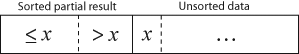
\includegraphics[width=8cm]{Insertionsort-before.png}
\end{figure}

\begin{figure}
		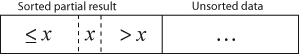
\includegraphics[width=8cm]{Insertionsort-after.png}
	\end{figure}


\begin{lstlisting}[language=c++, caption="Bubble-sort implementation in C++14"]
// CMP_FN has type: D -> D -> bool
template < typename Container, typename CMP_FN>
void insertionsort(Container& v, const int s,const int e, CMP_FN cmp) {
    for(int i=s+1 ; i<e; i++){
        int el = v[i];
        int j = i-1;
        while(cmp(el,v[j]) && j>=s){
            v[j+1] = v[j];
            j--;
        }
        v[j+1]=el;
    }
}
\end{lstlisting}

Suppose we have an array A, and that the subarray from index 0 through index $k$ is already sorted, and we want to insert the element currently in index $k+1$ into this sorted subarray, so that the subarray from index 0 through index $k+1$ is sorted. 
To insert the element in position $k+1$ into the subarray to its left, we repeatedly compare it with elements to its left , going right to left. Let's call the element in position $k+1$ the key. Each time we find that the key is less than an element to its left, we slide that element one position to the right, since we know that the key will have to go to that element's left. We'll need to do two things to make this idea work: we need to have a slide operation that slides an element one position to the right, and we need to save the value of the key in a separate place (so that it doesn't get overridden by the element to its immediate left). 

Here an Haskell implementation of \textit{insertion sort}
\begin{lstlisting}[language=Haskell,caption="Haskell Insertion sort "]
 insert :: Ord a => a -> [a] -> [a]
 insert item []  = [item]
 insert item (h:t) | item <= h = item:h:t
                   | otherwise = h:(insert item t)

 insertsort :: Ord a => [a] -> [a]
 insertsort []    = []   
 insertsort (h:t) = insert h (insertsort t)
\end{lstlisting}

\subsection{Complexity Analysis}
Time complexity is  $\mathcal{O}(n^2)$ while spatial complexity is  $\mathcal{O}(1)$. It is adaptive, and when each element does not move more than $k$ position from the original position to the sorted location its complexity is linear:  $\mathcal{O}(nk)$.   As for bubble-sort its best case is linear, but it performs much less operations mainly because bubble-sort is a \textit{exchange} algorithm while insertion sort is a \textit{shifting} one. Exchange requires a third of the operation of \textit{shifting}.

\section{Selection-Sort}
Selection sorting is conceptually the most simplest sorting algorithm. This algorithm first finds the smallest element in the array and exchanges it with the element in the first position, then find the second smallest element and exchange it with the element in the second position, and continues in this way until the entire array is sorted. 

The algorithm divides the input list into two parts: the sublist of items already sorted, which is built up from left to right at the front (left) of the list, and the sublist of items remaining to be sorted that occupy the rest of the list. Initially, the sorted sublist is empty and the unsorted sublist is the entire input list. The algorithm proceeds by finding the smallest (or largest, depending on sorting order) element in the unsorted sublist, exchanging (swapping) it with the leftmost unsorted element (putting it in sorted order), and moving the sublist boundaries one element to the right.

\begin{verbatim}
64 25 12 22 11 // this is the initial, starting state of the array

11 25 12 22 64 // sorted sublist = {11}

11 12 25 22 64 // sorted sublist = {11, 12}

11 12 22 25 64 // sorted sublist = {11, 12, 22}

11 12 22 25 64 // sorted sublist = {11, 12, 22, 25}

11 12 22 25 64 // sorted sublist = {11, 12, 22, 25, 64}
\end{verbatim}
\subsection{Complexity Analysis}
Time complexity is  $\mathcal{O}(n^2)$ and is generally slower than insertion sort and is not used in production code except when memory is very limited.





\section{Merge-Sort}
In computer science, merge sort (also commonly spelled mergesort) is an efficient, general-purpose, comparison-based sorting algorithm. Most implementations produce a stable sort, which means that the implementation preserves the input order of equal elements in the sorted output. Mergesort is a divide and conquer algorithm that was invented by John von Neumann in 1945.

Conceptually, a merge sort works as follows:
\begin{enumerate}
\item Divide the unsorted list into n sublists, each containing 1 element (a list of 1 element is considered sorted).
\item Repeatedly merge sublists to produce new sorted sublists until there is only 1 sublist remaining. This will be the sorted list.
\end{enumerate} 

Merge is the most important part of the algorithm. Merge algorithms are a family of algorithms that take multiple sorted lists as input and produce a single list as output, containing all the elements of the inputs lists in sorted order. These algorithms are used as subroutines in various sorting algorithms, most famously merge sort.

In particular merging two sorted collections into one can be done in linear time and linear space.When the inputs are linked lists, this algorithm can be implemented to use only a constant amount of working space; the pointers in the lists' nodes can be reused for bookkeeping and for constructing the final merged list.

\begin{lstlisting}[language=c++, caption="Bubble-sort implementation in C++14"]
// CMP_FN has type: D -> D -> bool
//[s1,e1] and [e1+1,e2] are two ordered sequences. This methods reaggarne the whole
// interval [s1,e2] in a sorted sequence
template < typename Container, typename CMP_FN>
void merge(Container& v, Container& scratch,  int s1,  int e1,  int e2,CMP_FN cmp){
    int s2 = e1+1;
    int ins =0;
    int b = s1;
    while(s1 <= e1 && s2<=e2)
        if(cmp(v[s1],v[s2]))
            scratch[b+ins++] = v[s1++];
        else
            scratch[b+ins++] = v[s2++];
    while(s1 <= e1)
        scratch[b+ins++] = v[s1++];
    while(s2 <= e2)
        scratch[b+ins++] = v[s2++];
        
    for(int i=0 ; i < ins ; i++)
        v[b+i] = scratch[b+i];
}
\end{lstlisting}

The following is the main mergesort method. It uses an helper function in order to hide the additional space required by the merge. Note that midpoint is computed using the \texttt{safe\_midpoint()} methods which avoids overflows for large $lo$ and $hi$ at a cost of an additional operation.

\begin{lstlisting}[language=c++, caption="Merge-sort"]
template<typename T>
inline T safe_midpoint(const T lo, const T hi){
    return lo+(hi-lo)/2;
}
template<typename T>
inline T unsafe_midpoint(const T lo, const T hi){
    return (hi+lo)/2;
}
#define TRIGGER_INSERTIONSORT (4)
template < typename Container, typename CMP_FN>
void mergesort_helper(Container& v,Container& scratch, const int s,const int e, CMP_FN cmp) {
    if(e -s <= TRIGGER_INSERTIONSORT)
        DS::insertionsort(v,s,e,cmp);
    if(s < e){
        int midpoint = safe_midpoint(s,e);
        mergesort_helper(v,scratch,s,midpoint,cmp);
        mergesort_helper(v,scratch,midpoint+1,e,cmp);
        merge(v,scratch,s,midpoint,e,cmp);
    }
}
// CMP_FN has type: D -> D -> bool
template < typename Container, typename CMP_FN>
void mergesort(Container& v, const int s,const int e, CMP_FN cmp) {
    Container scratch(v.size());
    mergesort_helper(v,scratch,s,e,cmp);

}
\end{lstlisting}


\textbf{QuickSort is better for contiguous data structures}.
In the merge sort algorithm, this subroutine is typically used to merge two sub-arrays $A[lo..mid]$, $A[mid..hi]$ of a single array $A$. This can be done by copying the sub-arrays into a temporary array, then applying the merge algorithm above.The allocation of a temporary array can be avoided, but at the expense of speed and programming ease. Various in-place merge algorithms have been devised, sometimes sacrificing the linear-time bound to produce an $\mathcal{nlog(n)}(n^2)$ algorithm.

Quick Sort in its general form is an in-place sort (i.e. it does not require any extra storage) whereas merge sort requires $O(N)$ extra storage, where $N$ denote the array size which may be quite expensive. Allocating and de-allocating the extra space used for merge sort increases the running time of the algorithm. Comparing average complexity we find that both type of sorts have $O(NlogN)$ average complexity but the constants differ (and sometimes matter). For arrays, merge sort loses due to the use of extra $O(N)$ storage space.

Most practical implementations of Quick Sort use randomized version. The randomized version has expected time complexity of O(nLogn). The worst case is possible in randomized version also, but worst case doesn’t occur for a particular pattern (like sorted array) and randomized Quick Sort works well in practice.
Quick Sort is also a cache friendly sorting algorithm as it has good locality of reference when used for arrays.
Quick Sort is also tail recursive, therefore tail call optimizations is done.

\textbf{Merge-Sort is better for Linked Data Structure}.
List case is different mainly due to differenc in memory allocation patterns w.t.r. to array.In linked list, we can insert items in the middle in $O(1)$ extra space and time. Therefore merge operation of merge sort can be implemented without extra space for linked lists (i.e. no waste of time during allocation and copy of any extra buffers). 
For contiguous data structure, we can do $O(1)$ time and space random access as elements are continuous in memory. But  Unlike arrays, we can not do random access in linked list \footnote{In linked list to access $i^{th}$ element, we have to travel each and every node from the head to $i^{th}$ node as we don not have continuous block of memory}. Quick Sort requires a lot of this kind of accesses. Therefore, the overhead increases for quick sort. Merge sort accesses data sequentially and the need of random access is low.


\subsubsection{Iterative Merge-Sort}

\subsection{Complexity Analysis}

Merge Sort is a recursive algorithm and time complexity can be expressed as following recurrence relation.
$T(n) = 2T(n/2) + \Theta(n)$
The above recurrence can be solved either using Recurrence Tree method or Master method. It falls in case II of Master Method and solution of the recurrence is $\Theta(nlog(n))$.
Time complexity of Merge Sort is $\Theta(nlog(n))$ in all 3 cases (worst, average and best) as merge sort always divides the array in two halves and take linear time to merge two halves.
Auxiliary Space: $O(n)$
Sorting In Place: No in a typical implementation
Stable: Yes




\section{Quick-Sort}

\subsection{Complexity Analysis}

\section{Heap-Sort}

\subsection{Complexity Analysis}

\section{Smoot-Sort}

\subsection{Complexity Analysis}


\section{Solving Recurrence relation}

\section{Substitution method}
\label{sec:substitutionmethod}
Despite the name, this is not a method that gives us a solution for the recurrence. It serves only to prove that an initial solution guess is right. It basically use induction to prove that the guess holds and is an actual solution of the recurrence equation.


\section{Recursion Tree method}
A recursion tree is useful for visualizing what happens when a recurrence is iterated. It diagrams the tree of recursive calls and the amount of work done at each call.
For instance, consider the recurrence
\[T(n) = 2T(\frac{n}{2}) + n^2\]
The recursion tree for this recurrence has the following form(see figure \ref{fig:rectree1})

\begin{figure}
\label{fig:rectree1}
		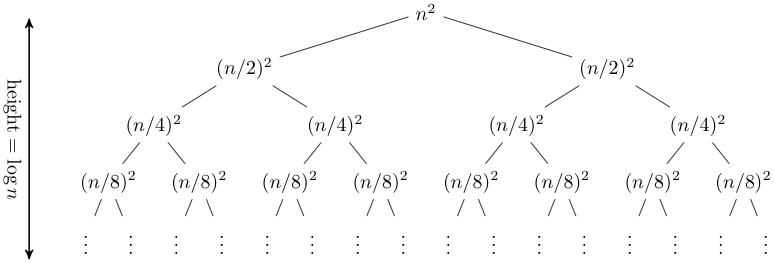
\includegraphics[width=12cm]{recTree1.png}
\end{figure}
It is easy to compute the amount of work done at each recursion level simply summing up all the nodes at a certain level (see figure \ref{fig:rectree2}).
\begin{figure}
\label{fig:rectree2}
		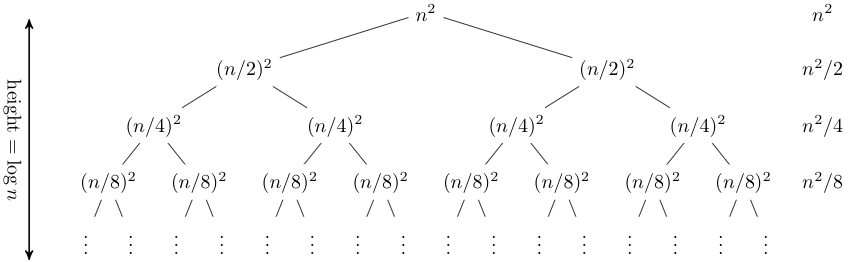
\includegraphics[width=12cm]{recTree2.png}
\end{figure}

In this case this is a geometric serie which sum limit is bounded by a quadratic function i.e. $O(n^2)$. 

Recursion trees can be useful for gaining intuition about the closed form of a recurrence, but they are not a proof (and in fact it is easy to get the wrong answer with a recursion tree, as is the case with any method that includes ''...'' kinds of reasoning). As we saw last time, a good way of establishing a closed form for a recurrence is to make an educated guess and then prove by induction that your guess is indeed a solution (see section \ref{sec:substitutionmethod} at page \ref{sec:substitutionmethod}). Recurrence trees can be a good method of guessing.


For example consider the following recurrence equation:
\[ T(n) = T(\frac{n}{3}) + T(\frac{2n}{3}) + n\]

Expanding the first levels of the corrensponding recursion tree we obtain the tree in figure \ref{fig:rectree3}.
\begin{figure}
\label{fig:rectree3}
		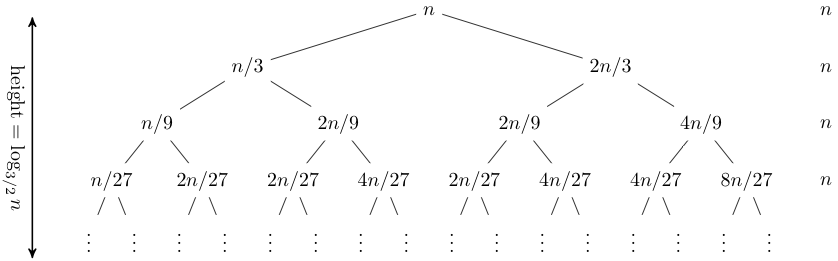
\includegraphics[width=12cm]{recTree3.png}
\end{figure}

Each level sums up to $n$, the height of this tree is $log_{\frac{3}{2}}(n)$. So out guess is that $T=O(nlogn)$.

Using the substitution method let's check if our guess is right.

\section{Master method}




\section{Questions \& Problems}
%---Question ------------
\begin{problem}
Which of the following is not a stable sorting algorithm in its typical implementation.
\begin{enumerate}
\item Insertion-sort
\item Merge-sort
\item Quick-sort
\item Bubble-sort
\end{enumerate}

\end{problem}

%---Question------------
\begin{problem}
Consider a situation where swap operation is very costly. Which of the following sorting algorithms should be preferred so that the number of swap operations are minimized in general?
\begin{enumerate}
\item Insertion-sort
\item Merge-sort
\item Quick-sort
\item Bubble-sort
\end{enumerate}

\end{problem}



%---Question------------
\begin{problem}
You have to sort 1 GB of data with only 100 MB of available main memory. Which sorting technique will be most appropriate?
\begin{enumerate}
\item Insertion-sort
\item Merge-sort
\item Quick-sort
\item Bubble-sort
\end{enumerate}

\end{problem}


%---Question------------
\begin{problem}
In a modified merge sort, the input array is splitted at a position one-third of the length(N) of the array. What is the worst case time complexity of this merge sort?
\begin{enumerate}
\item $\mathcal{O}(nlog_3(n))$
\item $\mathcal{O}(nlog_{\frac{2}{3}}(n))$
\item $\mathcal{O}(nlog_{\frac{1}{3}}(n))$
\item $\mathcal{O}(nlog_{\frac{3}{2}}(n))$

\end{enumerate}

\end{problem}


%---Question------------
\begin{problem}
Which sorting algorithm will take least time when all elements of input array are identical? Consider typical implementations of sorting algorithms.
\begin{enumerate}
\item Insertion-sort
\item Merge-sort
\item Quick-sort
\item Bubble-sort
\end{enumerate}

\end{problem}


%---Question------------
\begin{problem}
A list of n string, each of length n, is sorted into lexicographic order using the merge-sort algorithm. The worst case running time of this computation is:
\begin{enumerate}
\item $\mathcal{O}(nlog(n))$
\item $\mathcal{O}(n^2log(n))$
\item $\mathcal{O}(n^2 + log(n))$
\item $\mathcal{O}(n^2)$
\end{enumerate}

\end{problem}


%---Question1------------
\begin{problem}
Which of the following sorting algorithms has the lowest worst-case complexity?
\begin{enumerate}
\item Insertion-sort
\item Merge-sort
\item Quick-sort
\item Bubble-sort
\end{enumerate}

\end{problem}



%---Question1------------
\begin{problem}
Which of the following is true about merge sort?
\begin{enumerate}
\item Merge Sort works better than quick sort if data is accessed from slow sequential memory.
\item Merge Sort is stable sort by nature
\item Merge sort outperforms heap sort in most of the practical situations.
\item All the above.
\end{enumerate}

\end{problem}


%---Question1------------
\begin{problem}
Assume that a mergesort algorithm in the worst case takes 30 seconds for an input of size 64. Which of the following most closely approximates the maximum input size of a problem that can be solved in 6 minutes?
\begin{enumerate}
\item $2^8$
\item $2^9$
\item $2^{10}$
\item $2^{11}$
\end{enumerate}

\end{problem}



%---Problem------------
\begin{problem}
\textit{Given an array, write a program that prints 1 if array is sorted in non-decreasing order, else prints 0.}

\textbf{Input:}
The first line of input contains an integer $T$ denoting the number of test cases.
The first line of each test case contains $N$, which is the size of array (on the following line).
The second line of each test case contains $N$ input $C[i]$.

\textbf{Output:}
Print 1 if array is sorted, else print 0.

\textbf{Constraints:}
\begin{multline}\\
1 \leq T \leq 100\\
1 \leq N \leq 500\\
1 \leq C[i] \leq 1200\\
\end{multline}
\end{problem}

\begin{solution}
\begin{lstlisting}[language=C++, caption="C++ Solution"]
	int main(){
		return 0;	
	}
\end{lstlisting}

\end{solution}



%---Problem------------
\begin{problem}
\textit{Given a binary array, sort it in non-decreasing order.}

\textbf{Input:}
First line contains an integer denoting the test cases $T$.  Every test case contains two lines, first line is size $N$ and second line is space separated elements of array

\textbf{Output:}
Space separated elements of sorted arrays.  There should be a new line between output of every test case.

\textbf{Constraints:}
\begin{multline}\\
10 \leq T \leq 100\\
1 \leq N \leq 10000\\
\end{multline}

\textbf{Example:}
\begin{verbatim}
Input:
2
5
1 0 1 1 0
10
1 0 1 1 1 1 1 0 0 0

Output:
0 0 1 1 1
0 0 0 0 1 1 1 1 1 1 

\end{verbatim}

\end{problem}

\begin{solution}
\begin{lstlisting}[language=C++, caption="C++ Solution"]
	int main(){
		return 0;	
	}
\end{lstlisting}

\end{solution}



%---Problem------------
\begin{problem}
\textit{Given an array, print k largest elements from the array.}

\textbf{Input:}
The first line of input contains an integer $T$ denoting the number of test cases.
The first line of each test case is $N$ and $K$, where $N$ is the size of array and $K$ is the largest elements to be returned.
The second line of each test case contains $N$ input $C[i]$.

\textbf{Output:}
Print the $K$ largest elements in \textbf{descending order}.

\textbf{Constraints:}
\begin{multline}\\
10 \leq T \leq 50\\
1 \leq N \leq 100\\
K \leq N \\
1 \leq C[i] \leq 1000\\
\end{multline}

\textbf{Example:}
\begin{verbatim}
Input:
2
5 2
12 5 787 1 23
7 3
1 23 12 9 30 2 50

Output:
787 23
50 30 23

\end{verbatim}

\end{problem}

\begin{solution}
\begin{lstlisting}[language=C++, caption="C++ Solution"]
	int main(){
		return 0;	
	}
\end{lstlisting}

\end{solution}



%---Problem------------
\begin{problem}
Given an array with n distinct elements, convert the given array to a reduced form where all elements are in range from $[0 ... n-1]$. The order of elements is same, i.e., 0 is placed in place of smallest element, 1 is placed for second smallest element,\ldots $n-1$ is placed as last element.

\textbf{Input:}
The first line of input contains an integer $T$ denoting the number of test cases.
The first line of each test case is $N$, where $N$ is the size of array.
The second line of each test case contains $N$ input $A[i]$.

\textbf{Output:}
Print the reduced form of the array.

\textbf{Constraints:}
\begin{multline}\\
1 \leq T \leq 100\\
1 \leq N \leq 200\\
1 \leq A[i] \leq 500\\
\end{multline}

\textbf{Example:}
\begin{verbatim}
Input:
2
3
10 40 20
5
5 10 40 30 20

Output:
0 2 1
0 1 4 3 2

\end{verbatim}

\end{problem}


%---Problem------------
\begin{problem}
Given two array $A1$ and $A2$, sort $A1$ in such a way that the relative order among the elements will be same as those are in $A2$. For the elements not present in $A2$. Append them at last in sorted order.

\textbf{Input:}
The first line of input contains an integer $T$ denoting the number of test cases.
The first line of each test case is $M$ and $N,M$ are the number of elements in $A1$ and $A2$ respectively.
The second line of each test case contains $M$ elements.
The third line of each test case contains $N$ elements.
\textbf{Output:}
Print the sorted array according order defined by another array.

\textbf{Constraints:}
\begin{multline}\\
1 \leq T \leq 50\\
1 \leq N \leq M \leq 10\\
1 \leq A1[i],A2[i] \leq 500\\
\end{multline}

\textbf{Example:}
\begin{verbatim}
Input:
2
3
10 40 20
5
5 10 40 30 20

Output:
0 2 1
0 1 4 3 2

\end{verbatim}

\end{problem}


\begin{solution}
\begin{lstlisting}[language=C++, caption="C++ Solution"]
	int main(){
		return 0;	
	}
\end{lstlisting}

\end{solution}


%---Problem------------
\begin{problem}
\textit{Given an array of integers, sort the array according to frequency of elements. For example, if the input array is $\{2, 3, 2, 4, 5, 12, 2, 3, 3, 3, 12\}$, then modify the array to $\{3, 3, 3, 3, 2, 2, 2, 12, 12, 4, 5\}$}. 

If frequencies of two elements are same, print them in increasing order.

\textbf{Input:}
The first line of input contains an integer $T$ denoting the number of test cases. The description of $T$ test cases follows. The first line of each test case contains a single integer $N$ denoting the size of array. The second line contains $N$ space-separated integers $A1, A2, ..., AN$ denoting the elements of the array.

\textbf{Output:}
Print each sorted array on a newline. Each sorted array should be printed as space-separated.

\textbf{Constraints:}
\begin{multline}\\
1 \leq T \leq 70\\
1 \leq N \leq 130\\
1 \leq A[i] \leq 60\\
\end{multline}

\textbf{Example:}
\begin{verbatim}
Input:
1
5
5 5 4 6 4

Output:
4 4 5 5 6 

\end{verbatim}

\end{problem}

\begin{solution}
\begin{lstlisting}[language=C++, caption="C++ Solution"]
	int main(){
		return 0;	
	}
\end{lstlisting}

\end{solution}


%\chapter{Competitive Programming Problems}
\section{Common function functions }
This section describes the utility functions that are used to write solution for the followings problems.

\begin{lstlisting}[language=c++, caption="For each functions"]

template <typename Iterator, typename Lambda>
void for_each(Iterator s, Iterator e, Lambda l) {
  while (s != e) {
    l(*s);
    s++;
  }
}

//Lambda has type (T& -> int -> void)
template <typename Container, typename Lambda>
void for_each_i(Container& v, const int s, const int e, Lambda l) {
    int i=s;
    while (i < e){
        l(v[i],i);
        i++;
    }
}
	\end{lstlisting}
	
	
	
\begin{lstlisting}[language=c++, caption="Store credit c++ solution"]

template <typename T, typename Iterator>
bool contains(const Iterator s, const Iterator e, const T& value) {
  auto predicate_equal = [&](T curr) { return value == curr; };
  bool ret = e == find_if(s, e, predicate_equal);
  return !ret;
}

// Return value
// Iterator to the first element satisfying the condition or last if no such
// element is found.
template <typename Iterator, typename Lambda>
Iterator find_if(Iterator s, Iterator e, Lambda predicate) {
  while (s != e) {
    if (predicate(*s))
      return s;

    s++;
  }
  return e;
}

// Return value
// Iterator to the first element satisfying the condition or last if no such
// element is found.
template <typename Iterator, typename Lambda>
inline Iterator find_if_not(Iterator s, Iterator e, Lambda predicate) {
  auto not_predicate = [&](auto v) { return !predicate(v); };
  return find_if(s, e, not_predicate);
}

	\end{lstlisting}



\begin{lstlisting}[language=c++, caption="Store credit c++ solution"]
template <typename Iterator, typename Lambda>
bool all_of(Iterator s, Iterator e, Lambda predicate) {
  while (s != e) {
    if (!predicate(*s))
      return false;
    s++;
  }
  return true;
}

template <typename Iterator, typename Lambda>
bool any_of(Iterator s, Iterator e, Lambda predicate) {
  while (s != e) {
    if (predicate(*s))
      return true;
    s++;
  }

  return false;
}
\end{lstlisting}





\begin{lstlisting}[language=c++, caption="Store credit c++ solution"]
// Lambda has type: D -> T -> D
template <typename D, typename Iterator, typename Lambda>
D fold(Iterator s, Iterator e, const D& a, Lambda l) {
  D acc = a;
  while (s != e) {
    acc = l(acc, *s);
    s++;
  }
  return acc;
}

\end{lstlisting}


\begin{lstlisting}[language=c++, caption="Read input functions"]
template <typename T>
void readVector(std::vector<T>& v, const int size, std::istream& is=std::cin) {
  LOOPUP(i, size) {
    T a;
    is >> a;
    v.push_back(a);
  }
}

template <typename T, unsigned int D>
void readArray(std::array<T, D>& v, std::istream& is=std::cin) {
  LOOPUP(i, D) {
    T a;
    is>> a;
    v[i] = a;
  }
}


void read(auto& v, const unsigned int size, std::istream& is=std::cin) {
    using T=typename std::remove_reference<decltype(v[0])>::type;
  LOOPUP(i, size) {
    T a;
    is>> a;
    v[i] = a;
  }
}
\end{lstlisting}


\begin{lstlisting}[language=c++, caption="Store credit c++ solution"]
template<typename T>
inline T safe_midpoint(const T lo, const T hi){
    return lo+(hi-lo)/2;
}


template<typename T>
inline T unsafe_midpoint(const T lo, const T hi){
    return (hi+lo)/2;
}


template<typename T>
inline bool lt(const T& v1,const T& v2){
    return v1 < v2;
}

template<typename T>
inline bool eq(const T& v1,const T& v2){
    return v1 == v2;
}

template<typename T>
inline bool gt(const T& v1,const T& v2){
    return v1 > v2;
}

template<typename T>
inline bool gte(const T& v1,const T& v2){
    return gt(v1,v2) || eq (v1,v2);
}
template<typename T>
inline bool lte(const T& v1,const T& v2){
    return lt<T>(v1,v2) || eq<T>(v1,v2);
}

\end{lstlisting}




\begin{problem}{\textit{Store Credit} - \textbf{Google Jam Qualification Round Africa 2010}}
You receive a credit C at a local store and would like to buy two items. You first walk through the store and create a list L of all available items. From this list you would like to buy two items that add up to the entire value of the credit. The solution you provide will consist of the two integers indicating the positions of the items in your list (smaller number first).

\textbf{Input}

The first line of input gives the number of cases, N. N test cases follow. For each test case there will be:
One line containing the value C, the amount of credit you have at the store.
One line containing the value I, the number of items in the store.
One line containing a space separated list of I integers. Each integer P indicates the price of an item in the store. Each test case will have exactly one solution.

\textbf{Output}

For each test case, output one line containing "Case \#x: " followed by the indices of the two items whose price adds up to the store credit. The lower index should be output first.
\begin{framed}
	\begin{verbatim}
Input 
3
100
3
5 75 25
200
7
150 24 79 50 88 345 3
8
8
2 1 9 4 4 56 90 3

Output 
Case #1: 2 3
Case #2: 1 4
Case #3: 4 5
	\end{verbatim}
\end{framed}

\end{problem}

\begin{solution}
	
	\begin{lstlisting}[language=c++, caption="Store credit c++ solution"]

#include<common.h>
using namespace std;

int main(){
    using P=pair<int,int>;
    int N; cin>>N;

    LOOPUP(i,N){
        int C; cin>>C;
        int I; cin>>I;
        vector<int> items(I);
        vector<P> ip(I);
        DS::read(items,I);
        DS::for_each_i(ip,0,I,
            [&](auto& el, const int idx){el.first=items[idx]; el.second=idx;}
        );

        DS::quicksort(ip,0,I,DS::lt<P>);
        auto eq_fn = [](const P& p, const int v){ return p.first==v; };
        auto cmp_fn = [](const P& p, const int v){ return p.first<v; };
        LOOPUP(j,ip.size()){
            int val = (C-items[j]);
            int idx = DS::binary_search_idx(ip,0,ip.size(), val ,eq_fn,cmp_fn);
            //found. pickup the one with lowest INDEX
            if(idx!= -1){
                int retidx =idx;
                bool good=false;//check we do not pickup the same element twice
                while(eq_fn(ip[retidx],val) && j!= ip[retidx].second ){
                    retidx--;
                    good=true;
                }
                if(good){
                    int l = j+ 1;
                    int h = ip[retidx+1].second+1;
                    cout<<"Case #"<<i+1<<": "<<min(l,h)<<" "<<max(l,h)<<endl;
                    int sum = items[j] + items[ip[retidx+1].second];
                    assert(sum==C);
                    break;
                }
            }
        }
    }//foreach testcase
    return 0;
}

	\end{lstlisting}
\end{solution}





\begin{problem}{\textit{Rope Intranet} - \textbf{Google Jam Round 1C 2010}}

A company is located in two very tall buildings. The company intranet connecting the buildings consists of many wires, each connecting a window on the first building to a window on the second building.

You are looking at those buildings from the side, so that one of the buildings is to the left and one is to the right. The windows on the left building are seen as points on its right wall, and the windows on the right building are seen as points on its left wall. Wires are straight segments connecting a window on the left building to a window on the right building.

You've noticed that no two wires share an endpoint (in other words, there's at most one wire going out of each window). However, from your viewpoint, some of the wires intersect midway. You've also noticed that exactly two wires meet at each intersection point.

On the above picture, the intersection points are the black circles, while the windows are the white circles.

How many intersection points do you see?

\begin{figure}
\centering
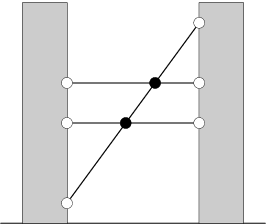
\includegraphics[scale=1]{ropeinternet}
\caption{}
\label{fig:ropeinternet}
\end{figure}

You've noticed that no two wires share an endpoint (in other words, there's at most one wire going out of each window). However, from your viewpoint, some of the wires intersect midway. You've also noticed that exactly two wires meet at each intersection point.

On figure \ref{fig:ropeinternet}, the intersection points are the black circles, while the windows are the white circles.

How many intersection points do you see?



\textbf{Input}
The first line of the input gives the number of test cases, T. T test cases follow. Each case begins with a line containing an integer N, denoting the number of wires you see.

The next N lines each describe one wire with two integers Ai and Bi. These describe the windows that this wire connects: Ai is the height of the window on the left building, and Bi is the height of the window on the right building.


\textbf{Output}
For each test case, output one line containing "Case \#x: y", where x is the case number (starting from 1) and y is the number of intersection points you see.

\begin{framed}
	\begin{verbatim}
Input 
2
3
1 10
5 5
7 7
2
1 1
2 2

Output 
Case #1: 2
Case #2: 0
	\end{verbatim}
\end{framed}

\end{problem}

\begin{solution}
	
	\begin{lstlisting}[language=c++, caption="Store credit c++ solution"]


	\end{lstlisting}
\end{solution}




\begin{problem}{\textit{Load Testing} - \textbf{Google Jam Round 1C 2010}}

Now that you have won Code Jam and been hired by Google as a software engineer, you have been assigned to work on their wildly popular programming contest website.

Google is expecting a lot of participants (P) in Code Jam next year, and they want to make sure that the site can support that many people at the same time. During Code Jam 2010 you learned that the site could support at least L people at a time without any errors, but you also know that the site can't yet support P people.

To determine how many more machines you'll need, you want to know within a factor of C how many people the site can support. This means that there is an integer a such that you know the site can support a people, but you know the site can't support a * C people.

You can run a series of load tests, each of which will determine whether the site can support at least X people for some integer value of X that you choose. If you pick an optimal strategy, choosing what tests to run based on the results of previous tests, how many load tests do you need in the worst case?



\textbf{Input}
The first line of the input gives the number of test cases, T. T lines follow, each of which contains space-separated integers L, P and C in that order.

\textbf{Output}
For each test case, output one line containing "Case \#x: y", where x is the case number (starting from 1) and y is the number of load tests you need to run in the worst case before knowing within a factor of C how many people the site can support.

\begin{framed}
	\begin{verbatim}
Input 
4
50 700 2
19 57 3
1 1000 2
24 97 2

Output 
Case #1: 2
Case #2: 0
Case #3: 4
Case #4: 2
	\end{verbatim}
\end{framed}

In Case \#2, we already know that the site can support between 19 and 57 people. Since those are a factor of 3 apart, we don't need to do any testing.

In Case \#4, we can test 48; but if the site can support 48 people, we need more testing, because $48*2 < 97$. We could test $49$; but if the site can't support $49$ people, we need more testing, because $24 * 2 < 49$. So we need two tests.

\end{problem}

\begin{solution}
	
This is a failry tricky problem.
	\begin{lstlisting}[language=c++, caption="Store credit c++ solution"]


	\end{lstlisting}
\end{solution}



\begin{problem}{\textit{File Fix-it} - \textbf{Google Jam Round 1B 2010}}

On Unix computers, data is stored in directories. There is one root directory, and this might have several directories contained inside of it, each with different names. These directories might have even more directories contained inside of them, and so on.

A directory is uniquely identified by its name and its parent directory (the directory it is directly contained in). This is usually encoded in a path, which consists of several parts each preceded by a forward slash ('/'). The final part is the name of the directory, and everything else gives the path of its parent directory. For example, consider the path:

\texttt{/home/gcj/finals}

This refers to the directory with name "finals" in the directory described by "/home/gcj", which in turn refers to the directory with name "gcj" in the directory described by the path "/home". In this path, there is only one part, which means it refers to the directory with the name "home" in the root directory.

To create a directory, you can use the mkdir command. You specify a path, and then mkdir will create the directory described by that path, but only if the parent directory already exists. For example, if you wanted to create the "/home/gcj/finals" and "/home/gcj/quals" directories from scratch, you would need four commands:
	\begin{verbatim}
mkdir /home
mkdir /home/gcj
mkdir /home/gcj/finals
mkdir /home/gcj/quals
	\end{verbatim}

\textbf{Given the full set of directories already existing on your computer, and a set of new directories you want to create if they do not already exist, how many mkdir commands do you need to use?}

\textit{No path will have more than 100 characters in it.
No path will appear twice in the list of directories already on your computer, or in the list of directories you wish to create. A path may appear once in both lists however. (See example case \#2 below).
If a directory is listed as being on your computer, then its parent directory will also be listed, unless the parent is the root directory.
The input file will be no longer than 100,000 bytes in total.
}

\textbf{Input}
The first line of the input gives the number of test cases, T. T test cases follow. Each case begins with a line containing two integers N and M, separated by a space.

The next N lines each give the path of one directory that already exists on your computer. This list will include every directory already on your computer other than the root directory. (The root directory is on every computer, so there is no need to list it explicitly.)

The next M lines each give the path of one directory that you want to create.

Each of the paths in the input is formatted as in the problem statement above. Specifically, a path consists of one or more lower-case alpha-numeric strings (i.e., strings containing only the symbols 'a'-'z' and '0'-'9'), each preceded by a single forward slash. These alpha-numeric strings are never empty.

\textbf{Output}
For each test case, output one line containing "Case \#x: y", where x is the case number (starting from 1) and y is the number of mkdir you need.

\begin{framed}
	\begin{verbatim}
Input 
3
0 2
/home/gcj/finals
/home/gcj/quals
2 1
/chicken
/chicken/egg
/chicken
1 3
/a
/a/b
/a/c
/b/b

Output 
Case #1: 4
Case #2: 0
Case #3: 4
	\end{verbatim}
\end{framed}

\end{problem}

\begin{solution}
	The idea behind this solution is to create a tree in which every possible path represents a different directory. The first N lines of the input are splitted and inserted in the tree. Then for each of M next  directories the code starting from the root try to find a path using the already present nodes. If this is not possible (a node with a certain label does not exists) then this directory does not exists and need to be created. It is then created and the procedure continues until the whole path is created. Every time a new node needs to be inserted a counter in incremented in order to keep track of the number of \texttt{mkdir} operations needed.
	
	\begin{lstlisting}[language=c++, caption="File fix it c++ solution"]
#include<common.h>
using namespace std;
class node{
public:
    string n;
    vector<node*> cs;
    bool done;

    node(){};
    node(string _n,bool _done = false): n(_n), done(_done) { }

    node* findChild(string s){
        auto f = [&](node* node){
            return ((node->n) == s);
        };
        auto ret = DS::find_if(cs.begin(),cs.end(),f);
        if(ret != cs.end())
            return *ret;
        return nullptr;
    }

    bool isLeaf(){
        return cs.size()==0;
    }
    ~node(){
        LOOPUP(i,cs.size()){
            delete cs[i];
        }
    }

};

void addNodes(vector<string> split, node* parent, bool val, int& count){
    if(split.size() > 0){
        string v = split.back();
        split.pop_back();
        node* present = parent->findChild(v);
        if(present)
            addNodes(split,present,val,count);
        else{
            //node not present create a new one
            if(val)
                count++;            

            node* n = new node(v,val && true);
            parent->cs.push_back(n);
            addNodes(split,n,val,count);
        }
    }

}


#define CLRSS(ss) ss.clear(); ss.str("");

int main(){
    int T; cin>>T;
    LOOPUP(i,1,T+1){
        int N,M; cin>>N>>M;
        cin.ignore(std::numeric_limits<std::streamsize>::max(),'\n');
        //cout<<N<<" "<<M<<endl;
        node* root = new node();
        stringstream ss;
        auto foldsplit = [&](auto* split, char c){
            if(c=='/'){
                split->push_back(ss.str());
                CLRSS(ss);
            }else{
                ss<<c;
            }
            return split;
        };

        int count = 0;
        //alreadypresent
        LOOPUP(j,N){
            string s; cin>>s;
            s=s.substr(1,s.size());
            vector<string> split;
            DS::fold(ALL(s),&split,foldsplit);
            split.push_back(ss.str());
            DS::reverse(split,split.size());
            CLRSS(ss);
            addNodes(split,root,false,count);
        }

        //create
        LOOPUP(j,M){
            string s; cin>>s;
            s=s.substr(1,s.size());
            vector<string> split;
            DS::fold(ALL(s),&split,foldsplit);
            split.push_back(ss.str());
            DS::reverse(split,split.size());//reverse in order to pop_back efficently
            CLRSS(ss);
            addNodes(split,root,true,count);
        }
        printf("Case #%d: %d\n",i,count);

        delete root;
    }

    return 0;
}

	\end{lstlisting}
\end{solution}

\begin{problem}{\textit{Rope Intranet} - \textbf{Google Jam Round 1C 2010}}




\textbf{Input}


\textbf{Output}


\begin{framed}
	\begin{verbatim}
Input 


Output 

	\end{verbatim}
\end{framed}

\end{problem}

\begin{solution}
	
	\begin{lstlisting}[language=c++, caption="Store credit c++ solution"]


	\end{lstlisting}
\end{solution}



\begin{problem}{\textit{Rope Intranet} - \textbf{Google Jam Round 1C 2010}}




\textbf{Input}


\textbf{Output}


\begin{framed}
	\begin{verbatim}
Input 


Output 

	\end{verbatim}
\end{framed}

\end{problem}

\begin{solution}
	
	\begin{lstlisting}[language=c++, caption="Store credit c++ solution"]


	\end{lstlisting}
\end{solution}



\begin{problem}{\textit{Rope Intranet} - \textbf{Google Jam Round 1C 2010}}




\textbf{Input}


\textbf{Output}


\begin{framed}
	\begin{verbatim}
Input 


Output 

	\end{verbatim}
\end{framed}

\end{problem}

\begin{solution}
	
	\begin{lstlisting}[language=c++, caption="Store credit c++ solution"]


	\end{lstlisting}
\end{solution}



\begin{problem}{\textit{Rope Intranet} - \textbf{Google Jam Round 1C 2010}}




\textbf{Input}


\textbf{Output}


\begin{framed}
	\begin{verbatim}
Input 


Output 

	\end{verbatim}
\end{framed}

\end{problem}

\begin{solution}
	
	\begin{lstlisting}[language=c++, caption="Store credit c++ solution"]


	\end{lstlisting}
\end{solution}



\begin{problem}{\textit{Rope Intranet} - \textbf{Google Jam Round 1C 2010}}




\textbf{Input}


\textbf{Output}


\begin{framed}
	\begin{verbatim}
Input 


Output 

	\end{verbatim}
\end{framed}

\end{problem}

\begin{solution}
	
	\begin{lstlisting}[language=c++, caption="Store credit c++ solution"]


	\end{lstlisting}
\end{solution}

%----------------------------------------------------------------------------------------
%	BIBLIOGRAPHY
%----------------------------------------------------------------------------------------

\chapter*{Bibliography}
\addcontentsline{toc}{chapter}{\textcolor{ocre}{Bibliography}}
\section*{Books}
\addcontentsline{toc}{section}{Books}
\printbibliography[heading=bibempty,type=book]
\section*{Articles}
\addcontentsline{toc}{section}{Articles}
\printbibliography[heading=bibempty,type=article]

%----------------------------------------------------------------------------------------
%	INDEX
%----------------------------------------------------------------------------------------

\cleardoublepage
\phantomsection
\setlength{\columnsep}{0.75cm}
\addcontentsline{toc}{chapter}{\textcolor{ocre}{Index}}
\printindex

%----------------------------------------------------------------------------------------



%\backmatter

\end{document}
